\chapter{State of Art}%
\label{chapter:stateofart}

%  mantain this? 
% \begin{introduction}
% In this chapter, the evolution leading to Industry 5.0 contextualizes the importance of technological advancements. 
% The focus is on Industry 5.0, particularly its transition from autonomous robots to the emerging dynamics of \ac{HRC}.
% The critical need for collaborative scenarios between humans and robots is highlighted, emphasizing the transformative potential of such partnerships. 
% Moreover, the integration of digital realities with \ac{DT} in Industry 5.0 is evaluated for its impact on enhancing \ac{HRI}, signaling a new era of efficiency and 
% collaboration in industrial operations.
% \end{introduction}
* TODO: Add introduction to the chapter - paragraph with 2/3 lines explaining core concepts that will be discussed in the chapter - confirm this

\section{Key Drivers of Industry 5.0}
\label{section:industry-evolution}
With the advent of Industry 4.0 and the emerging concept of Industry 5.0, the industry environment has witnessed significant transformations. Understanding this progress is crucial to contextualize the technological advancements and the shift towards more human-centric manufacturing processes.

\subsection{Industry 4.0: The Fourth Industrial Revolution}

Industry 4.0 represents the integration of cutting-edge digital technologies into manufacturing processes, leading to the emergence of smart factories. It leverages advanced systems such as \ac{CPSS}, the \ac{IoT}, robotics, \ac{AR}, simulation, cloud computing, and big data analytics, as illustrated in Figure~\ref{fig:key-tech-industry-4}. This paradigm signifies a fundamental shift towards interconnected, intelligent, and digitally-driven manufacturing ecosystems, revolutionizing the way products are conceived, manufactured, and delivered, while enhancing production efficiency, flexibility, and innovation~\cite{Moller2022, Ahmed2022}.

\begin{figure}[!htbp]
    \centering
    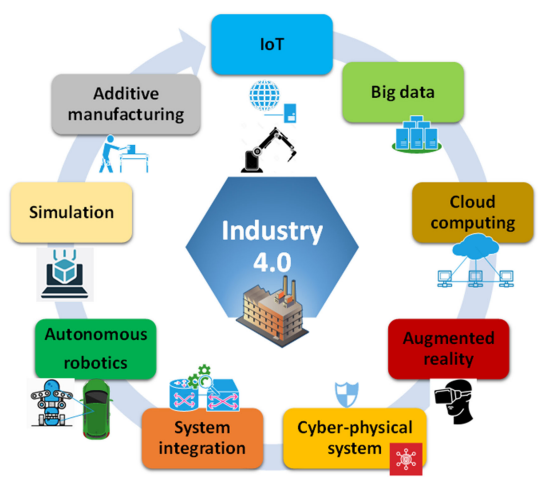
\includegraphics[width=0.7\linewidth]{figs/key-tech-industry-4.png}
    \caption{Key enabling technologies in Industry 4.0~\cite{Ahmed2022}}
    \label{fig:key-tech-industry-4}
\end{figure}
\FloatBarrier

With advancements in \ac{AI}, industrial processes can achieve unprecedented performance levels, often exceeding human capabilities. These \ac{AI}-driven systems enable robots to perform tasks that may be too hazardous, complex, or delicate for humans, such as handling dangerous materials or managing microscopic elements. Despite this extraordinary potential, it is important to recognize that current industrial robots are not as "smart" as humans in many contexts and, even though these robots are capable of performing highly skilled tasks, they frequently operate under strict, pre-programmed limits~\cite{Ahmed2022}.

Although Industry 4.0 has undoubtedly increased productivity, flexibility, and automation in industrial environments, it has also led to concerns regarding the diminishing role of human operators. This relentless push towards full automation has, in some cases, reduced human involvement in critical decision-making processes, leading to a more machine-centric production landscape~\cite{GOLOVIANKO2023102}.

\subsection{Industry 5.0: Reintegrating the Human Element}

Approximately a decade after the launch of Industry 4.0, the European Commission introduced the Industry 5.0 concept in response to new societal challenges~\cite{industry5}. The growing concerns about the exclusion of human operators in Industry 4.0 systems, coupled with the limitations of full automation, paved the way for this new industrial paradigm. Industry 5.0 seeks to reintroduce the human element into industrial ecosystems, emphasizing greater human involvement in manufacturing processes~\cite{su11164371}.

The main goal consists on combining the strengths of humans and machines to achieve more sustainable, efficient, and human-centered production systems. This shift reflects the realization that, while machines excel at repetitive, dangerous, or complex tasks, humans provide irreplaceable creativity, adaptability, and problem-solving abilities~\cite{10577684}. Industry 5.0 aims to strike a balance between technological advancement and human-centric values, fostering environments where humans work alongside advanced technologies to achieve greater societal and environmental outcomes~\cite{GOLOVIANKO2023102}.


% While Industry 4.0 focused on pushing the limits of automation and data-driven production, Industry 5.0 reintroduces the importance of human collaboration. 
Recognizing that humans and machines each possess distinct strengths that can complement one another, the following key technological drivers of Industry 5.0 build upon the advancements of Industry 4.0~\cite{10577684}:
%  These drivers signify a shift towards greater human-machine collaboration, addressing the limitations of full automation while fostering more adaptive, intelligent, and human-centric industrial systems.

\begin{itemize}
    \item \textbf{Collaborative Robots (Cobots):} are engineered to ensure safe, collaborative operation alongside human workers, facilitating not only intuitive interactions but also fostering efforts that leverage the unique strengths of both humans and robots. Their integration is driven by the need to create systems that enable seamless, user-friendly \ac{HRC}, in full alignment with the guiding principles of Industry 5.0. This paradigm shift redefines traditional employment roles by emphasizing \ac{HRI}, with a focus on communication and coordination with robotic systems and advanced \ac{AI}.

    \item \textbf{Digital Twins:} represent a pivotal technological advancement in Industry 5.0. They provide visual models that enhance comprehension and facilitate the evaluation of goods, processes, and production systems. By allowing real-time monitoring and simulation, \ac{DT} help optimize manufacturing processes, bridging the gap between the virtual and physical worlds.

    \item \textbf{Human-Centric Automation:} Emphasis is placed on using technology to augment human capabilities rather than replace them, fostering a more inclusive, creative, and flexible manufacturing environment. This approach ensures that technology empowers human workers, enabling them to focus on tasks requiring intuition and creativity.

    \item \textbf{Advanced Human-Machine Interfaces:} The development of intuitive interfaces, by integrating technologies such as \ac{AR} and \ac{VR}, facilitates better communication between humans and machines. These interfaces allow for more natural interactions, improving understanding and efficiency in collaborative tasks.

    \item \textbf{Artificial Intelligence and Cognitive Computing:} These technologies continue to evolve, enabling robots and automation systems to work alongside humans in ways that enhance productivity without fully replacing them. \ac{AI} allows for more intuitive \ac{HMI}, where machines can understand and respond to human needs more effectively.

    \item \textbf{Sustainable and Resilient Manufacturing:} Industry 5.0 also focuses on sustainability and resilience, integrating environmental considerations into manufacturing processes. This includes optimizing resource usage and reducing waste, aligning technological advancement with ecological responsibility.
\end{itemize}

By integrating these key drivers, Industry 5.0 addresses the challenges identified in Industry 4.0, promoting harmonious collaboration between humans and machines. This synergy aims to enhance productivity while preserving the unique contributions of human workers, ultimately leading to more innovative, sustainable, and human-centered industrial practices.


% %%%%%%%%%%%%%%%%%%%%%%%%%%%%%%%%%%%%%%%%%%%%%%%%%%%%%%%%%%%%%%%%

% \section{Introduction to Industry 5.0} As a response to the increasing automation and the need for greater human involvement in manufacturing 
% processes, "Industry 5.0" seeks to reintroduce the human element into industrial ecosystems. Unlike Industry 4.0, which prioritized automation and 
% machine autonomy, Industry 5.0 emphasizes human-robot collaboration, where the strengths of humans and machines are combined to achieve more sustainable, 
% efficient, and human-centered production systems. This shift reflects the realization that while machines excel at repetitive, dangerous, or complex tasks,
% humans provide irreplaceable creativity, adaptability, and problem-solving abilities.

% Industry 5.0 seeks to strike a balance between technological advancement and human-centric values, fostering environments where humans work alongside 
% advanced technologies to achieve greater societal and environmental outcomes \cite{GOLOVIANKO2023102}.

\section{Human-Robot Collaboration}
%%%% estender um pouco mais e fazer ponte para collaboration scenarios / digital realities
\label{subsection:human-robot-collab}
% \input{chapters/stateofart/subsections/human-robot-collab}

The field of \ac{HRI} is dedicated to examining the interactions and coexistence of humans and robots in shared spaces, whose objective consists on enhancing these interactions by designing robots that are safe, effective and compatible for assisting and cooperating with humans in diverse roles, rather than replacing them \cite{Ogenyi2021}.
This involves developing robots that are, not only autonomous, but also capable of understanding and communicating with humans, as well as predicting
human-behavior and learning from human feedback. 

However, \ac{HRI} can be broken down into different forms of interaction, whose categorization is based on various factors that define how 
humans and robots share the workspace. This disctinction is represented in the Figure \ref{fig:collab} and can be broken down into \textbf{Coexistence}, \textbf{Cooperation} and \textbf{Collaboration} \cite{Jahanmahin2022}. 
Each one can be distinguished by the degree of interaction and task sharing between humans and robots:

* TODO: center the figure - it is but since the table is too wide, it seems not to be centered
\begin{figure}[!htbp]
    % \centering
    % \hspace{-1.3cm}
    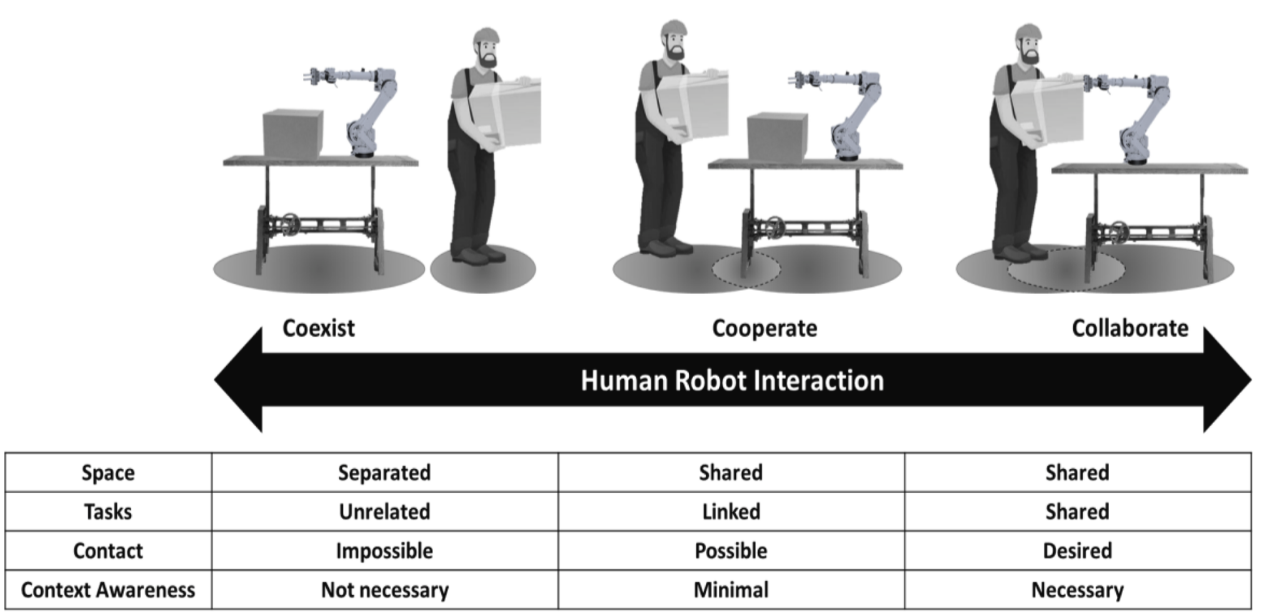
\includegraphics[width=\linewidth]{figs/collab-coex-coopr.png}
    \caption{Different levels of \ac{HRI}~\cite{Jahanmahin2022}} 
    \label{fig:collab}
\end{figure} 

\begin{itemize}
    \item \textbf{\ac{HRCx}}: In this form of interaction, humans and robots operate in the same environment but perform entirely independent tasks without interaction. The workspace is separated, there is no contact, and context awareness is unnecessary since the tasks are unrelated.
    Usually this interaction does not involve synchronized work or communication between the two parties. 

    \item \textbf{\ac{HRCp}}: Here, humans and robots share the workspace and work on linked tasks, towards a common goal. Advanced technologies such as sensors or machine vision may be used to detect and prevent collisions. Contact is possible, though not essential and actions are largely independent  with occasional coordinated efforts.

    \item \textbf{Human-Robot Collaboration (\ac{HRC})}: represents the most advanced and integrated form of \ac{HRI}. In \ac{HRC}, humans and robots not only share a common workspace but also actively collaborate on shared objectives. This collaboration can involve direct physical contact, such as the joint manipulation of objects, or non-physical interaction, including verbal communication, gestures, or pattern recognition.
    Within such environments, humans often handle tasks that require fine motor skills, decision-making, or creative problem-solving, while robots take on repetitive, strenuous, or hazardous activities, ensuring efficiency and safety. This synergy enhances productivity by leveraging the unique strengths of both humans and robots, creating a dynamic partnership where each complements the other’s capabilities.

\end{itemize}

In the bottom part of the Figure \ref{fig:collab} there is a table that further breaks down these distinctions, highlighting key factors like space, task relationship, possibility of contact, and the need for context awareness. This gradient from coexistence to collaboration shows the increasing complexity and interdependence in \ac{HRI}, as technology evolves to make robots more capable partners in industrial and service environments.

% explanation of the below figure
Below, the Figure \ref{fig:hrc-workstation} illustrates a \ac{HRC} workspace, showcasing the interaction between a human worker and a robot within a shared environment. The workspace is divided into distinct yet overlapping areas: the robot's work envelope and the human's work envelope. These areas reflect the respective tasks of each party, with the robot likely performing repetitive or automated tasks, such as material handling within the feeding system, while the human focuses on more intricate tasks requiring dexterity and decision-making.

The overlapping shared workspace demonstrates the core principle of \ac{HRC}, where humans and robots work together toward common goals, necessitating real-time coordination and communication. In this setup, advanced sensing technologies or machine vision are essential to ensure safety and prevent collisions, allowing both the human and robot to operate efficiently within close proximity.

This image underscores how robots, rather than replacing humans, complement human skills by taking on routine, physically demanding tasks, while humans contribute with their cognitive abilities. This partnership reflects the broader vision of Industry 5.0, where human creativity and robotic precision are combined to create adaptable, human-centered industrial processes, enhancing both efficiency and safety in collaborative environments.

\begin{figure}[!htbp]
    \centering
    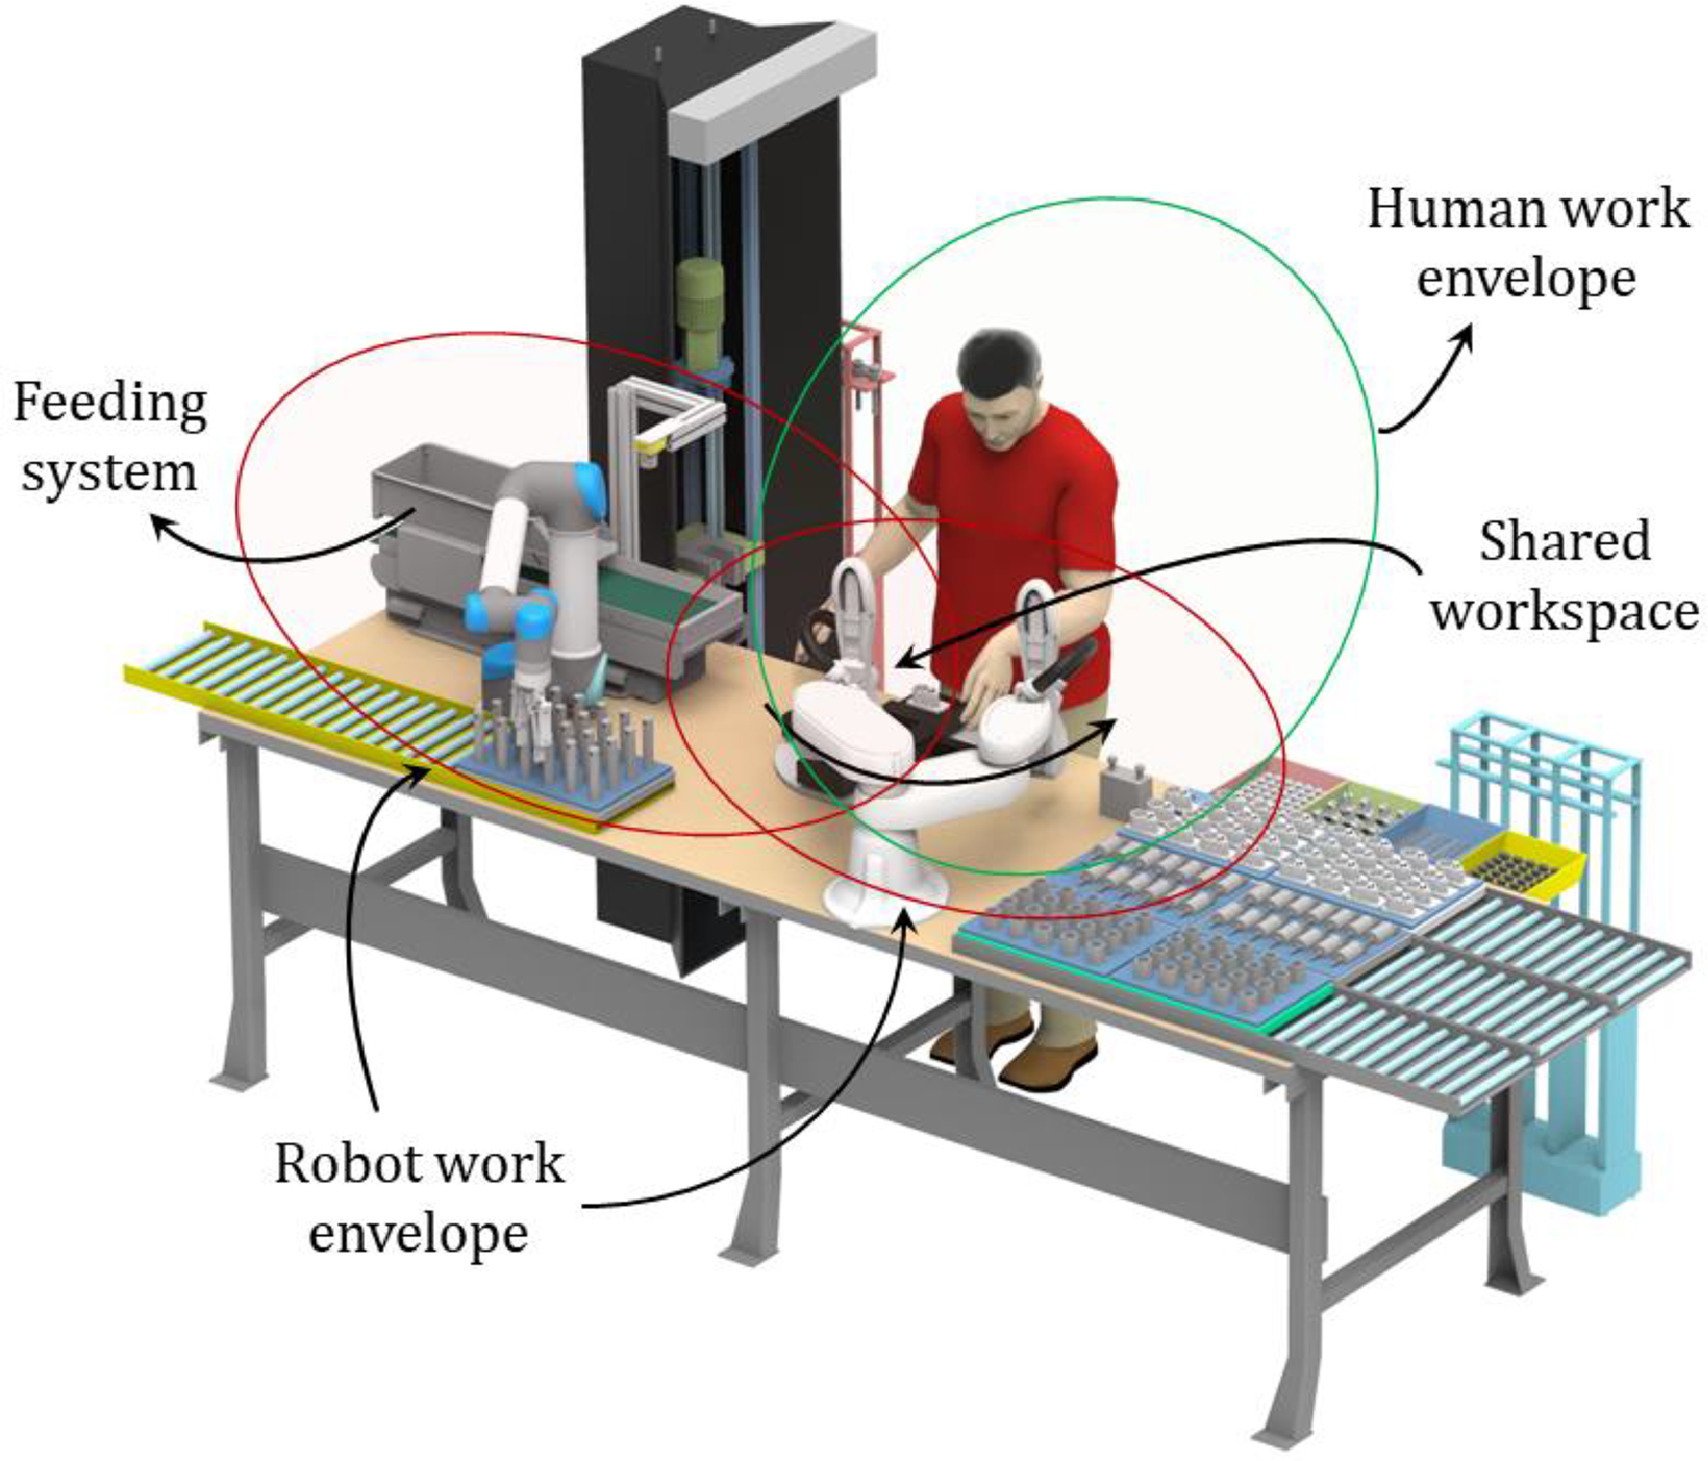
\includegraphics[width=0.55\linewidth]{figs/workspace-station-high-res-image.jpg}
    \caption{Workstation example enabling collaboration between human and robot while sharing the same physical space~\cite{MALIK2021102092}} 
    \label{fig:hrc-workstation}
\end{figure} 

%  link do artigo com a figura: https://www.sciencedirect.com/science/article/pii/S0736584520303021#fig0002
%  workspace-station-high-res-image - figura com alta resolução
%  workspace-station-full-image - figura full size

These new robots featuring intelligent sensing and vision systems, envisioned to integrate the production line, are called "cobots". 
They represent the alternative to full automation, since industry specialists have stated it is not possible to completely remove the 
human within the manufacturing environment \cite{Weiss2021}.

%% adicionar figura correta e dar label - verificar depois esta questao do estado da arte aqui

%%%%%%%%%%%%%%%%%%%%%%%% analise do artigo sobre cobots - Human–Robot Collaboration in Manufacturing Applications: A Review - 2019
%%%%%%%%%%%%%%%%%%%%%%%% ver melhor esta parte abaixo, organizar melhor e adicionar referencias bem, imagens e o que está a faltar
\section{Collaborative Robots (Cobots)} 

The concept of collaborative robots, or "cobots," was first introduced by J. Edward Colgate and Michael Pashkin in 1996 \cite{cobot-definition}, laying the foundation for practical applications in \ac{HRC}. Cobots are designed to physically interact with humans in shared workspaces, without the need for protective barriers typical in traditional robotic systems. This innovation paved the way for a new category of robots that excel in adaptability and flexibility, although effective use requires a deep understanding of their unique characteristics \cite{robotics8040100}.

\begin{figure}[!htbp]
    \centering
    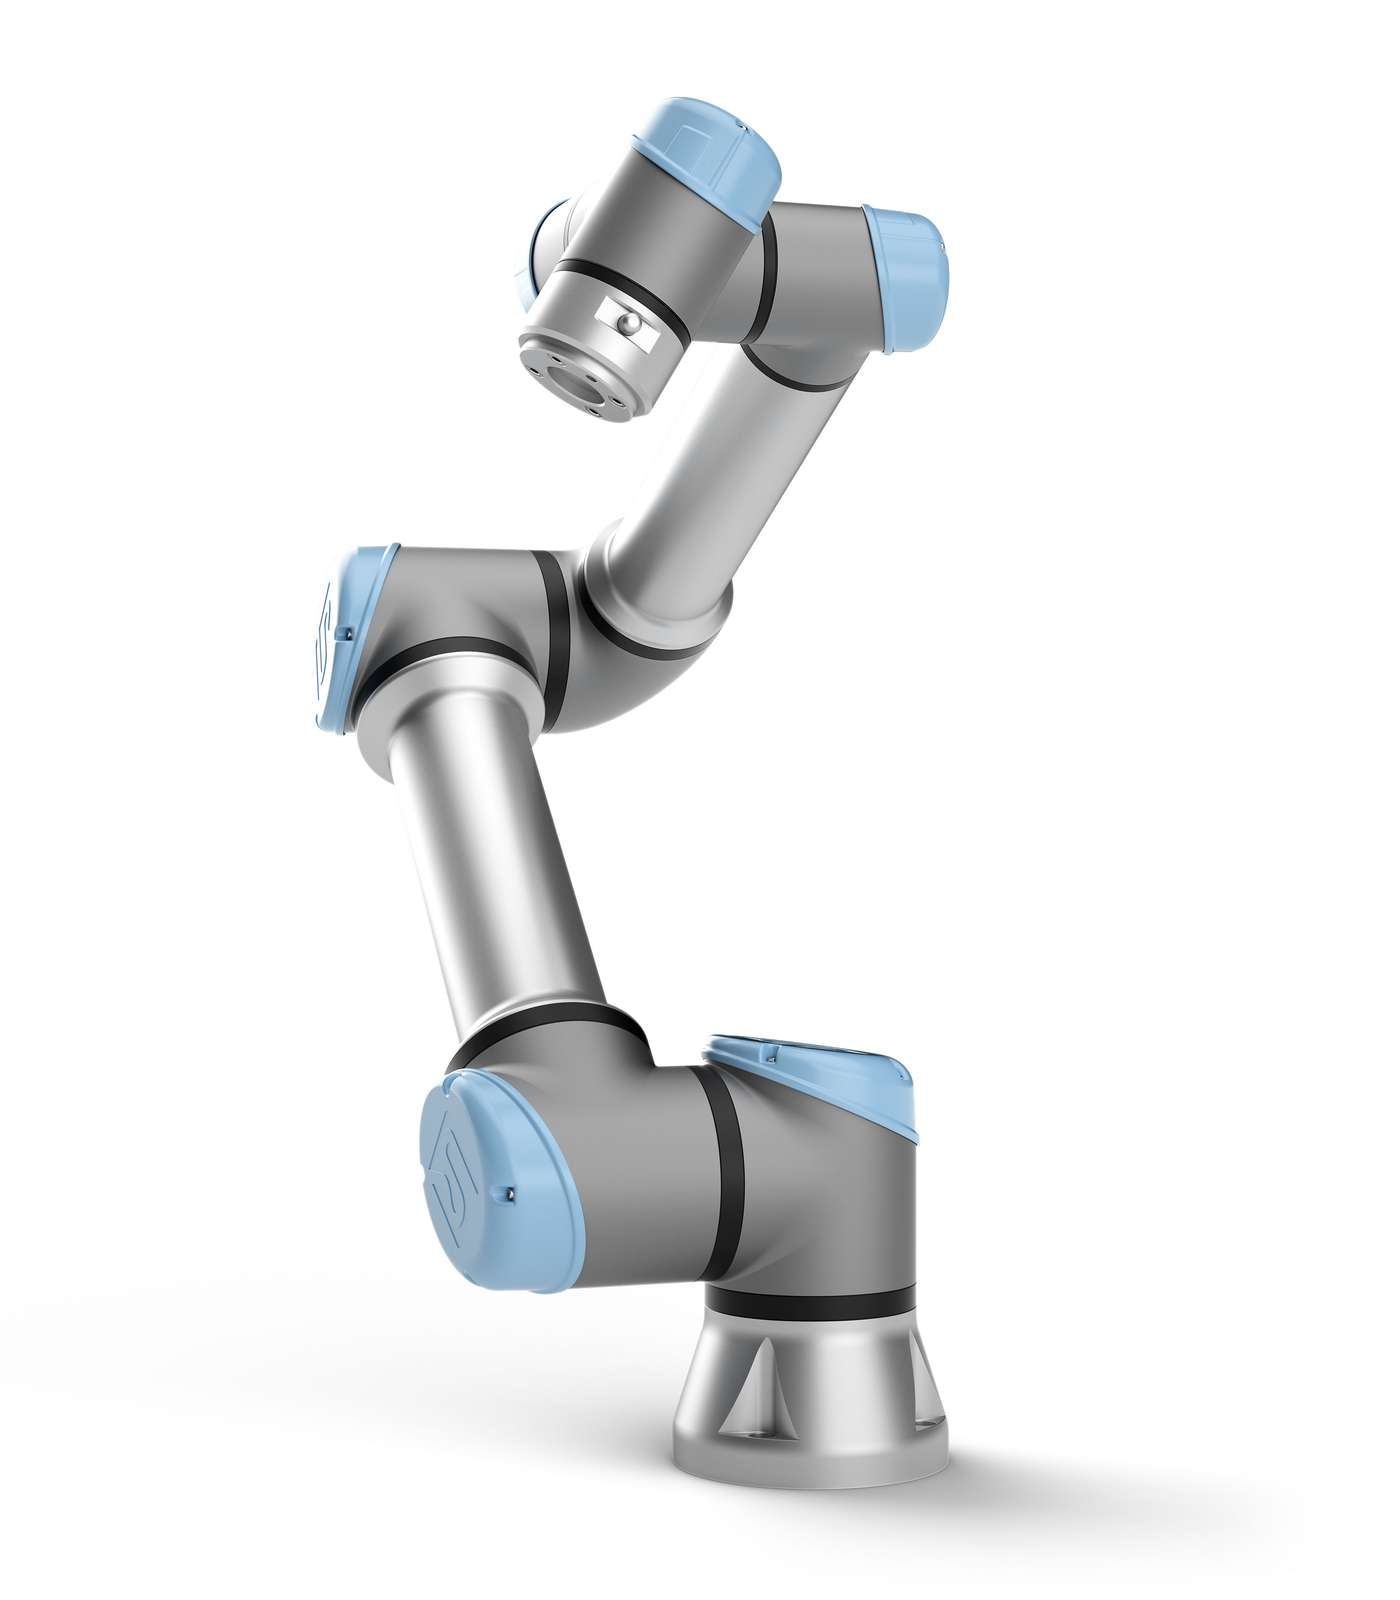
\includegraphics[width=0.4\linewidth]{figs/ur5.jpg}
    \caption{Universal Robots UR5 cobot} 
    \label{fig:ur5}
\end{figure} 

Commercializing cobots began in 2008 with the release of the UR5 model by Universal Robots, marking a breakthrough in \ac{HRC} technologies and facilitating the integration of cobots into industrial workflows \cite{robotics8040100}. The UR5, shown in Figure~\ref{fig:ur5}, represents a pivotal development in collaborative robotics, as it enabled quicker and more cost-effective adaptation of industrial layouts.

% \subsubsection{The Role and Benefits of Cobots}

Unlike traditional industrial robotic systems, which require extensive safety guarding and consequently reduce flexibility while increasing both costs and spatial demands, cobots present a solution tailored to the current market's demand for shorter lead times and mass customization, particularly for \ac{SMEs} \cite{barbazza2017agility}.

This cobots' emergence represents a paradigm shift in industrial automation, emphasizing \ac{HRC} over the traditional model of robotic isolation. These facilitate direct physical interaction between humans and machines while being designed for intuitive use, enabling even non-experts to reprogram them effortlessly \cite{7140065}. By leveraging the complementary strengths of human cognitive capabilities and robotic precision, cobots offer substantial productivity gains and reduced operational costs.

% \subsubsection{Background and Evolution of Cobots}



% \subsubsection{Distinguishing Cobots from Industrial Robots}

Cobots differentiate themselves from traditional industrial robots by prioritizing safety, ergonomics, and user accessibility. Unlike conventional robots that require extensive safety enclosures, cobots are equipped with advanced features such as force and torque sensors, vision systems, and anti-collision mechanisms. These capabilities enable them to operate safely in close proximity to humans without the need for restrictive barriers \cite{cobots-design}. The inherent design of cobots supports flexibility and ease of deployment, avoiding the high costs and complexity associated with retrofitting traditional robotic systems for similar functionality.

% \subsubsection{Economic and Practical Advantages of Cobots}

The adoption of cobots in industrial settings is driven by a combination of economic, operational, and health-related factors:
\begin{itemize}
    \item \textbf{Cost Efficiency:} Cobots can significantly reduce labor costs by performing repetitive tasks, thereby lowering direct unit production costs compared to traditional automation solutions \cite{cobot-2019collaborative}.
    \item \textbf{Enhanced Workplace Safety:} Their design minimizes occupational hazards, which leads to improved worker safety and health, addressing ergonomic challenges in manual labor.
    \item \textbf{Spatial Efficiency:} The compact and flexible nature of cobots allows them to be easily relocated and reconfigured within different production areas, optimizing factory space utilization \cite{cobots-implementation}.
\end{itemize}


These attributes are particularly beneficial in high-risk applications and industries that demand frequent changes in production layouts, such as electronics, automotive, and aerospace manufacturing.

When assessing the applicability of cobots versus traditional robots, several distinctions emerge. Cobots excel in tasks that require adaptability and human-like dexterity, such as assembly, placement, handling, and quality inspection. Their versatility and ease of integration make them suitable for low-volume, high-mix production environments, where agility is crucial. However, traditional robots retain an advantage in scenarios that demand high payload capacity, speed, and precision, particularly in heavy-duty manufacturing applications \cite{robotics8040100}.

Despite their advantages, integrating cobots still encounters challenges for some use-cases. Issues such as interoperability with legacy systems, programming complexity for non-standard tasks, and optimizing cobot performance in dynamic environments require further research and development. Additionally, advancements in \ac{AI} and \ac{ML} could unlock new capabilities for cobots, enabling them to autonomously adapt to changing tasks and work conditions, thereby extending their utility beyond predefined, structured environments.

Moreover, \ac{MR} technologies are becoming increasingly pivotal in advancing cobot integration, offering immersive, real-time interfaces that enhance \ac{HRC}. By overlaying digital information onto the physical workspace, \ac{MR} facilitates better situational awareness and task execution for both operators and cobots. Coupled with \ac{DT} systems, \ac{MR} enables real-time monitoring and control of cobots in dynamic and remote settings, enhancing operational flexibility. Integrating \ac{MR} into cobot applications thus allows for more intuitive interactions, improved safety, and higher precision in collaborative environments. As part of Industry 5.0, these technologies collectively contribute to creating more responsive, human-centered manufacturing systems.
%%%%%%%%%%%%%% 16set 18h04 a parte abaixo, está ok ver so se é preciso adicionar mais alguma figura
\section{Digital Realities} 
\ac{DRs} encompass a wide spectrum of technologies that merge virtual elements with real-world environments to varying extents. In 1994, Milgram and Kishino introduced the Reality-Virtuality Continuum, a theoretical framework that characterizes the progression from a purely physical environment to a fully virtual one, as illustrated in Figure \ref{f:real-virtual-continuum} \cite{milgram1994}.
This continuum is divided into four principal stages: Reality, \ac{AR}, \ac{AV}, and \ac{VR}.

\begin{figure}[h]
    \centering
    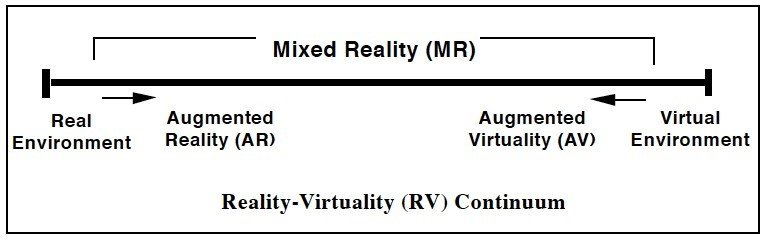
\includegraphics[width=0.7\linewidth]{figs/vr-continuum.png}
    \caption{Reality-Virtuality Continuum~\cite{milgram1994}}
    \label{f:real-virtual-continuum}
\end{figure}

In this continuum, Reality represents the perception of an unaltered physical environment, devoid of any virtual modifications. As we progress along the continuum towards the virtual side, different digital realities offer increasingly immersive experiences by blending or replacing real-world content with virtual elements.

\subsection{Augmented Reality}
    \ac{AR} enhances a user's interaction with their physical environment by overlaying dynamic digital content, such as 3D objects, information layers, or media, onto the real world \cite{liu2022digitaltwin}. The main goal of \ac{AR} is to seamlessly integrate virtual objects with the user's surrounding physical context, facilitating real-time interaction between the virtual and physical realms allowing users to experience both virtual and real entities as coexisting within the same space, generating a cohesive and interactive environment \cite{Azuma1997}.
    
    Figure \ref{f:ar-example} \footnote{\url{https://www.cad-schroer.de/news-events/artikel/mixed-reality-augmented-reality-virtual-reality-definition-und-uebersicht/}, Acessed: 2024-10-19} provides a clear representation of \ac{AR} being employed in an industrial maintenance scenario. The user views real-time digital overlays on a physical machine, providing essential information such as the machine’s current status and highlighting critical components for maintenance or repair. This visual guidance significantly enhances the user’s understanding of tasks by seamlessly blending virtual instructions with the real environment, thereby improving efficiency and reducing the potential for human error.

    \begin{figure}[!htpb]
        \centering
        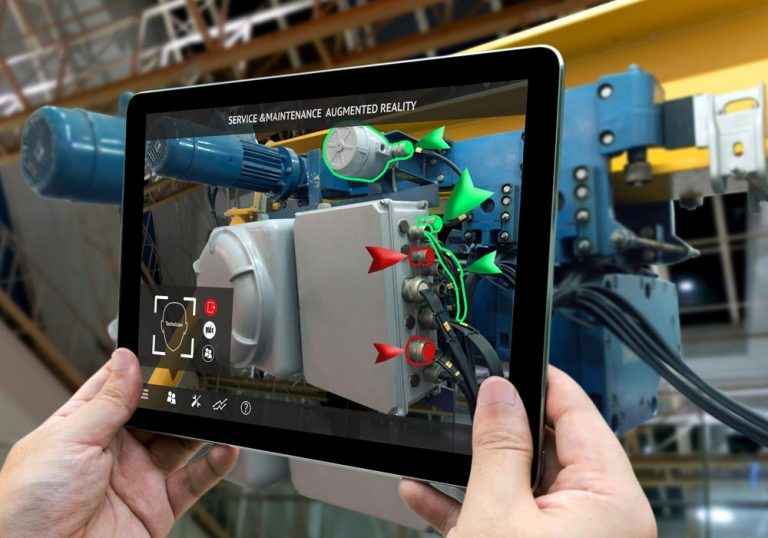
\includegraphics[width=0.6\linewidth]{figs/ar-example.jpg}
        \caption{Augmented Reality application of industry overlayed information in order to assist the operator}
        \label{f:ar-example}
    \end{figure}

    Achieving this level of integration requires accurate spatial registration, a process that ensures that virtual elements are properly aligned with real-world objects in both location and scale. The spatial coherence between the two realities is critical for creating an effective \ac{AR} experience, where virtual objects respond to changes in the environment and user interaction in real-time. 

    Various \ac{AR} devices are employed to deliver these experiences, including \ac{AR}-\ac{HMDs}, tablets, \ac{HHDs}, projectors, and see-through \ac{VR} headsets with built-in cameras. Each device offers different degrees of environmental awareness and interaction capabilities, such as hand tracking and holographic projection. 
    % These technologies have transformed numerous industries, offering new possibilities in fields ranging from manufacturing and design to healthcare and entertainment.

    * TODO: add more references to the above 2 paragraphs

\subsection{Virtual Reality}
    
    Within the Reality-Virtuality Continuum proposed by Milgram and Kishino, \ac{VR} occupies the extreme end of the spectrum, representing a complete substitution of a user’s perception of the physical world with a fully immersive synthetic environment. In this state, the user is entirely isolated from their real surroundings, perceiving only the artificially constructed virtual environment, typically presented through a range of immersive devices such as \ac{HMDs} \cite{milgram1994}. Figure~\ref{f:real-virtual-continuum} \footnote{\url{https://en.wikipedia.org/wiki/Immersion_\%28
    virtual_reality\%29\#/media/File:Reality_check_ESA384313.jpg}} illustrates this immersive experience where the user interacts with a virtual environment through \ac{VR} equipment.

    \begin{figure}[h]
        \centering
        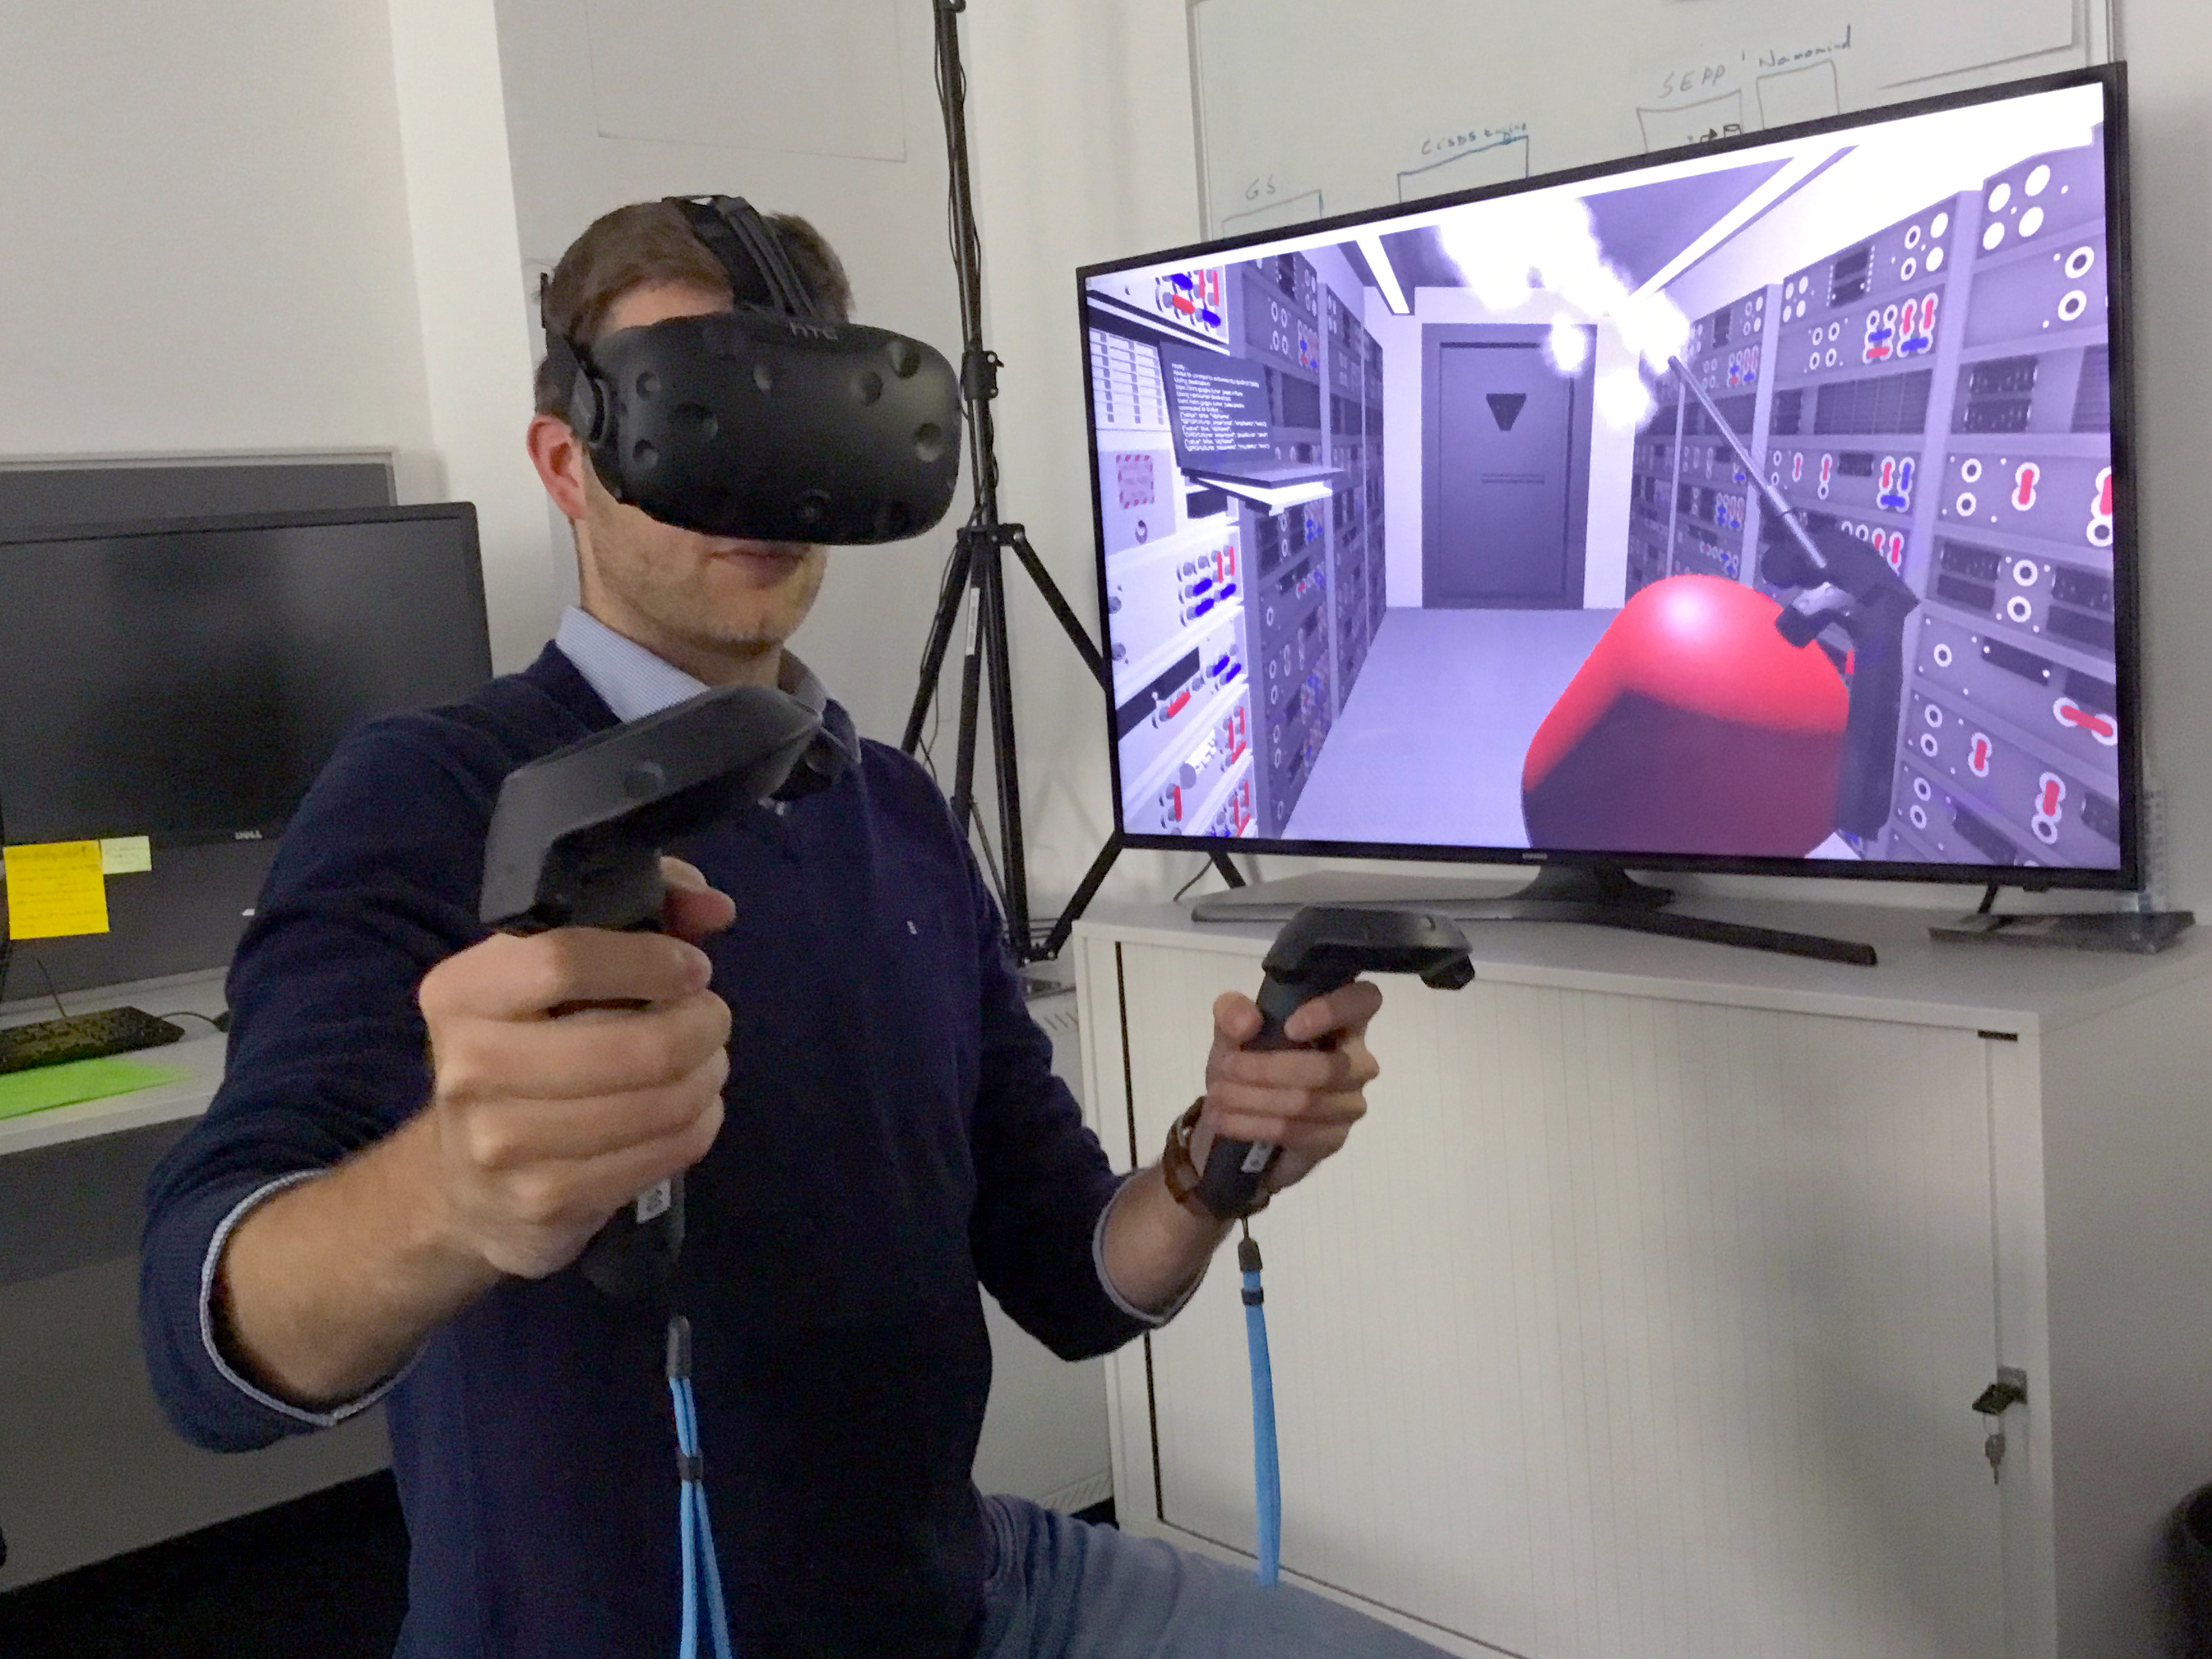
\includegraphics[width=0.6\linewidth]{figs/Reality_check_ESA384313.jpg}
        \caption{User immersed in a virtual environment using a VR headset, demonstrating complete isolation from the physical world.}
        \label{f:real-virtual-continuum}
    \end{figure}

    Modern \ac{VR} systems achieve this full immersion by leveraging advanced \ac{HMDs}, which present stereoscopic images directly to the user’s eyes through built-in displays or projection systems. These devices often incorporate additional features like head tracking, enabling the user’s head movements to influence their viewpoint in the virtual environment, further enhancing the sense of immersion and presence \cite{whatismixedreality}. Some systems also include positional tracking through external sensors or inside-out tracking via integrated cameras, allowing users to physically navigate virtual spaces, augmenting both interaction fidelity and spatial awareness.

    \ac{VR} is particularly effective in applications that require the user to be completely enveloped in an artificial environment, thus enabling the simulation of real-world scenarios, historical reconstructions, or entirely imaginative worlds. This sense of "presence," wherein users perceive the virtual environment as real, is fundamental to \ac{VR}'s efficacy across various domains, including gaming, education, training, and simulation. Additionally, \ac{VR}'s potential to create deeply immersive and isolated experiences makes it especially valuable in fields like remote collaboration, where users can interact with simulated environments or models that are otherwise inaccessible \cite{8712803}.

    * TODO: add more references here  

    % \begin{figure}[h]
    %     \centering
    %     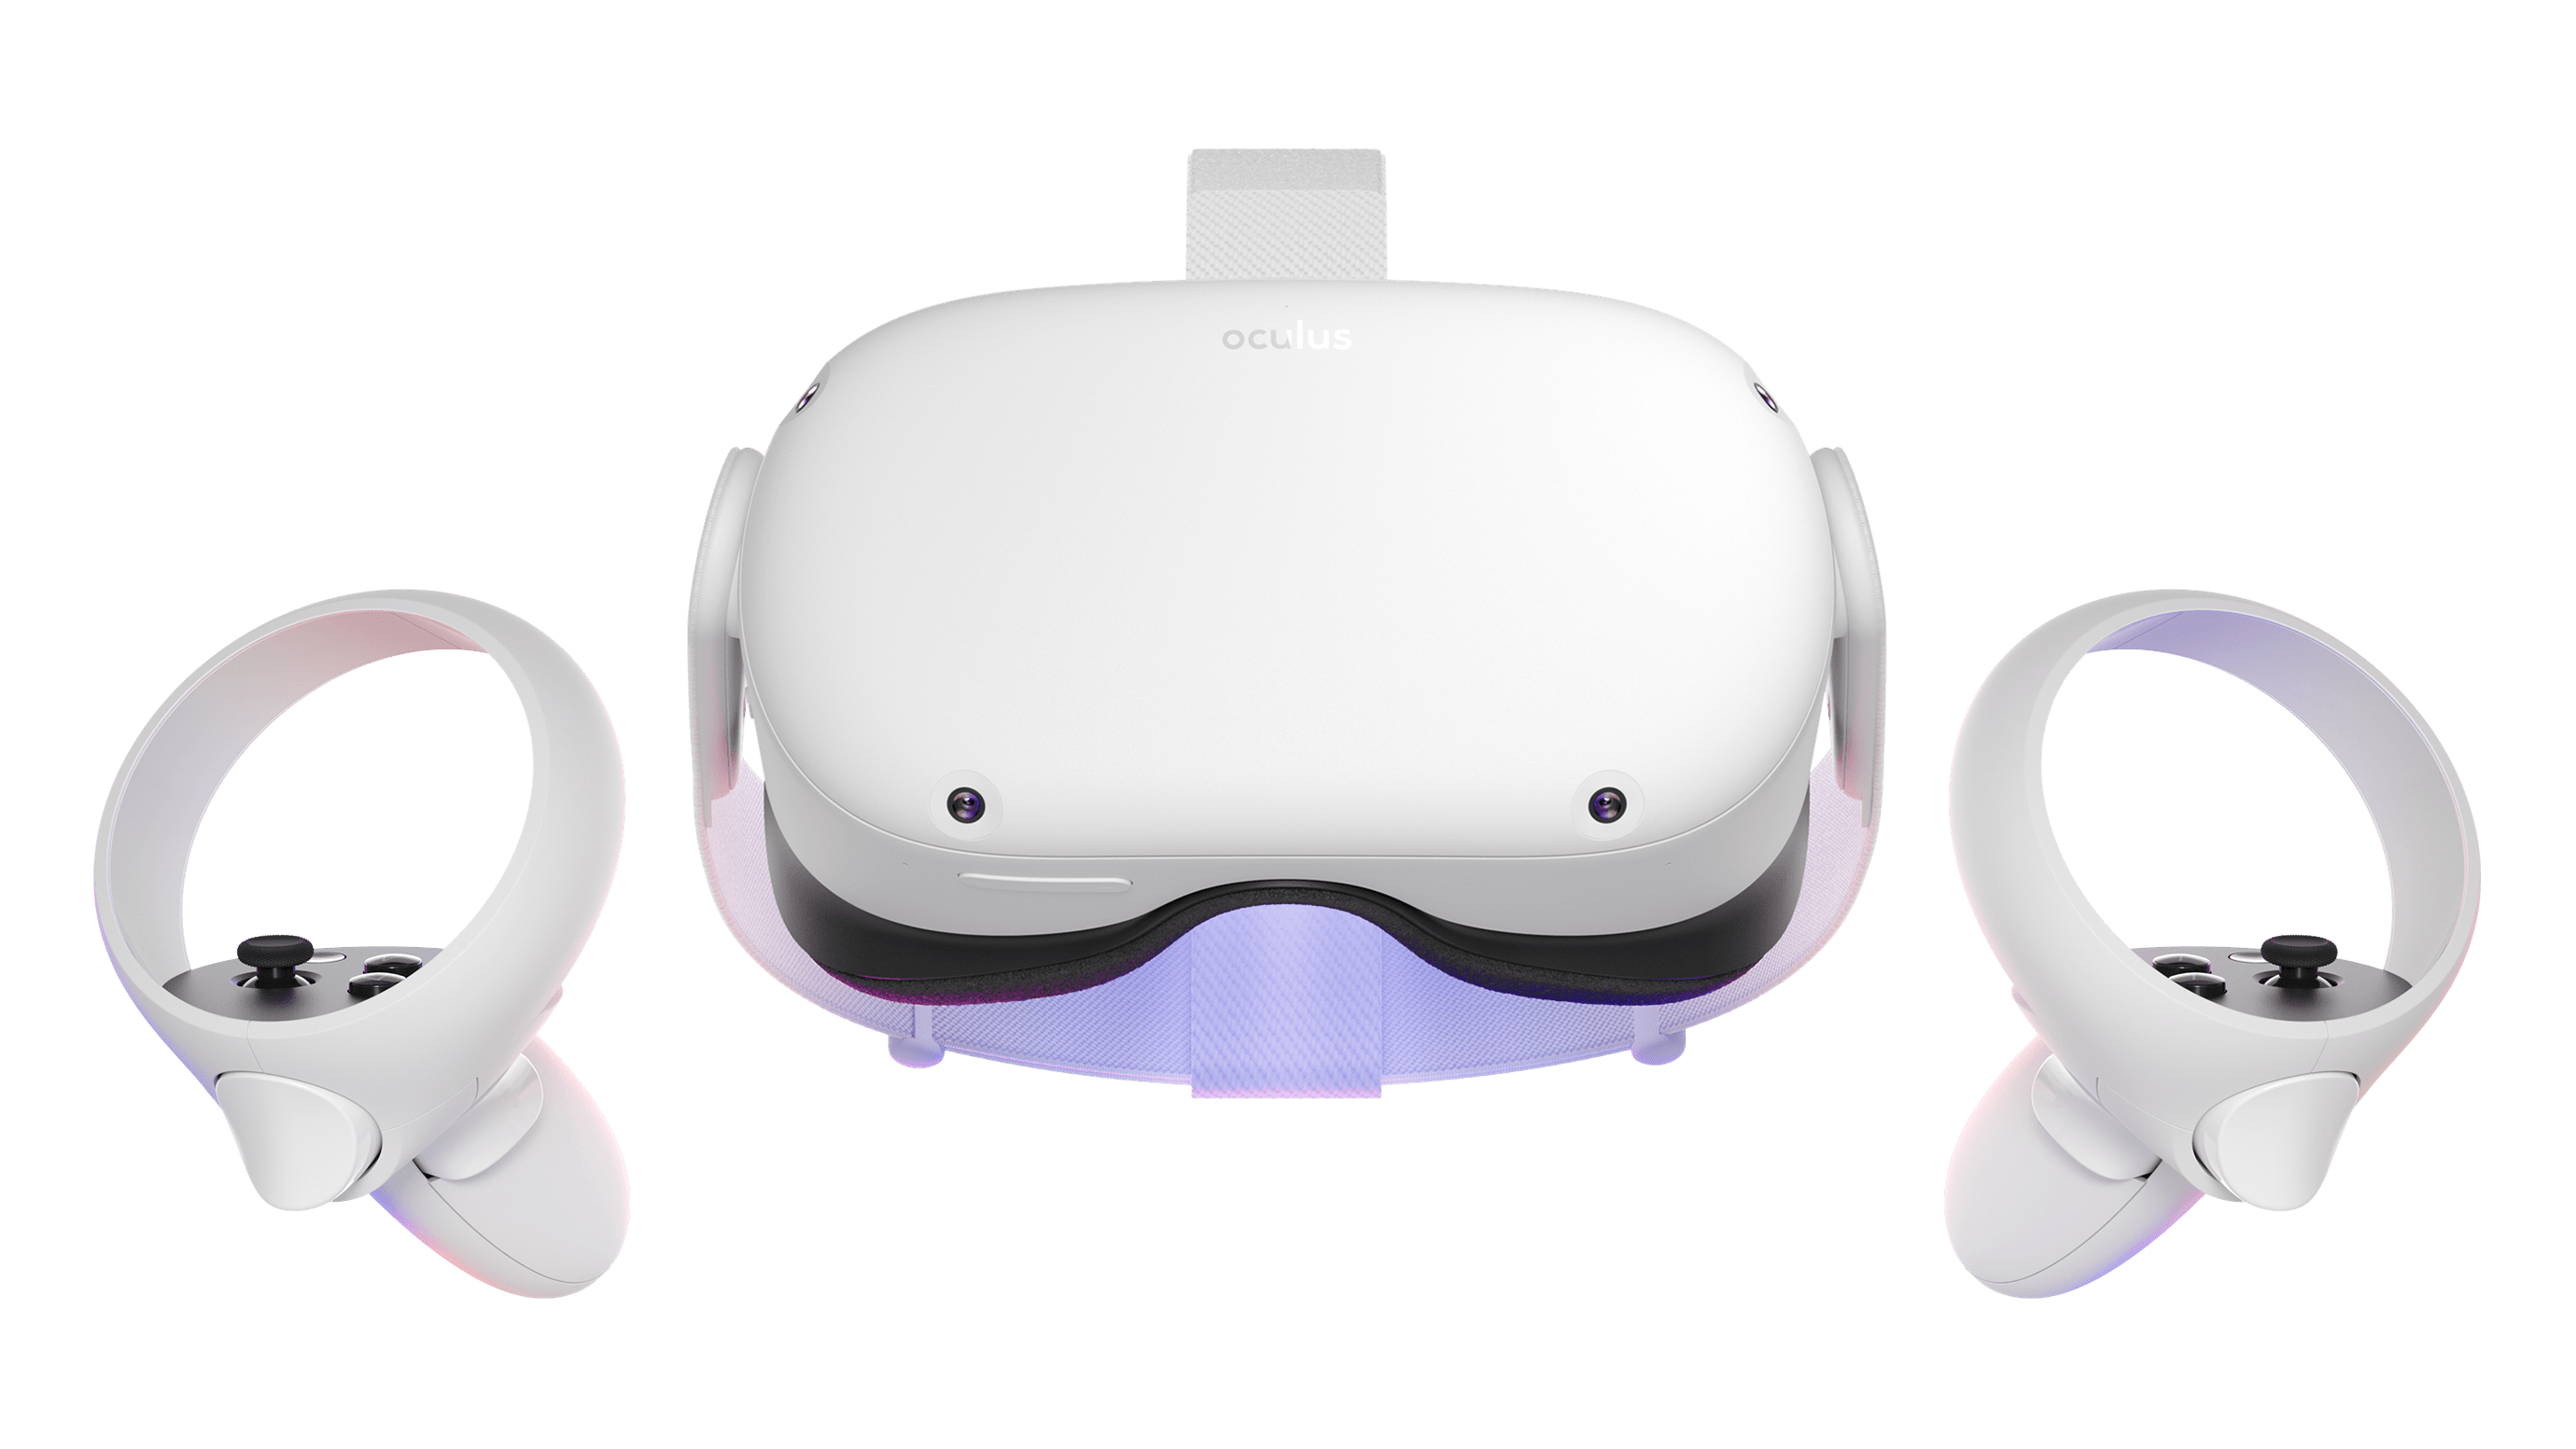
\includegraphics[width=0.6\linewidth]{figs/oculus-2-vr.png}
    %     \caption{Oculus Quest headset}
    %     \label{f:quest-2-vr}
    % \end{figure}

\subsection{Mixed Reality}
\label{subsection:digital-realities}
   
    \ac{MR} continues to elude a universally accepted definition, with interpretations diverging significantly across academic and industrial domains. According to the Milgram and Kishino Reality-Virtuality Continuum, depicted in Figure \ref{f:real-virtual-continuum}, \ac{MR} occupies a transitional space between \ac{AR} and \ac{AV}, bridging the two concepts \cite{milgram1994}. Expanding on this, Microsoft’s \ac{MR} spectrum defines \ac{MR} as spanning a range of technologies, from \ac{AR} (where physical reality predominates, augmented with digital overlays) to \ac{AV} (where the virtual environment dominates, supplemented by real-world data) \cite{microsoft_mixed_reality}. 

    * TODO: ADD REFERENCES IN BELOW TEXT
    In \ac{MR} environments, digital and physical elements coexist and interact in real time, creating a dynamic interface where virtual and physical worlds seamlessly blend. This enables immersive, bi-directional interaction, where users engage with both digital objects and real-world elements, facilitating fluid communication between virtual entities and the physical environment. This integration enhances the user experience by enabling virtual objects to influence, and be influenced by, real-world contexts in a highly interactive manner, enabling new forms of collaboration, visualization, and interaction.

    The inherent complexity of \ac{MR} arises from the challenge of ensuring a natural and intuitive integration of digital and physical elements. This requires advanced environmental sensing, real-time data fusion, and contextual understanding to deliver interactions that appear natural to the user. 
    % Consequently, the hardware requirements for \ac{MR} are more demanding than those for \ac{AR} or \ac{VR} alone. \ac{MR} systems typically employ spatial computing techniques, integrating high-fidelity sensors, advanced computational algorithms, and computer vision to recognize and map physical spaces, thus allowing for more sophisticated interactions.

    Despite considerable advancements, the definition of \ac{MR} remains contested. Speicher et al. (2019) identified six competing notions of \ac{MR} across both scholarly literature and industry practice, underscoring the fragmentation in its interpretation. Some experts argue that \ac{MR} represents an enhanced form of \ac{AR}, where users are not merely passive observers but active participants interacting with a responsive augmented space. In this interpretation, \ac{MR} is seen as a "stronger" form of \ac{AR}, exemplified by technologies such as Microsoft's HoloLens, where users can manipulate virtual elements within their physical environment \cite{whatismixedreality}.

    Other perspectives view \ac{MR} as a convergence of \ac{AR} and \ac{VR}, where the boundary between the real and virtual worlds is fluid and adaptable, creating immersive, hybrid experiences. For example, the widely known game Pokémon Go is sometimes cited as an \ac{MR} application, where a \ac{VR}-based digital environment enables users to interact with augmented digital elements such as Pokémons, overlaid onto the physical world \cite{whatismixedreality}.

    However, the definition most relevant to this project's development emphasizes \ac{MR} as a powerful medium for collaboration, enabling users to interact across different realities—whether physical, augmented, or virtual. In this context, \ac{MR} facilitates shared experiences between users located in distinct environments. For example, a physical space visualized by an on-site \ac{AR} user can be simultaneously recreated and experienced by a remote \ac{VR} user, allowing real-time collaborative interactions between participants situated in different realities. This capacity for cross-reality collaboration enhances both the user’s understanding of the workspace and the efficiency of the collaboration process.

    An example of this collaborative interaction is depicted in Figure \ref{f:mr-example-collab}, where a trainer (remote) and trainee (on-site) engage in a task that bridges physical and virtual worlds. In this scenario, the trainee uses \ac{VR} technology to operate within a virtual environment, while the trainer remotely observes and provides guidance. Through this setup, the trainer can not only visualize the trainee's actions but also trigger events or scenarios via a dedicated interface, enhancing the learning experience. This type of interaction exemplifies the capabilities of remote training, where an expert can guide an on-site operator using real-time augmented indications displayed on \ac{AR} glasses or tablets. By providing direct visual and auditory feedback, the remote trainer assists in troubleshooting, guiding the trainee through complex tasks or maintenance operations. This form of collaboration allows geographically distant participants to work synchronously in a highly interactive environment, increasing both efficiency and accuracy in training processes \cite{Mayer2023}.
  
    % Mayer2023 referencia da figura
    \begin{figure}[h]
        \centering
        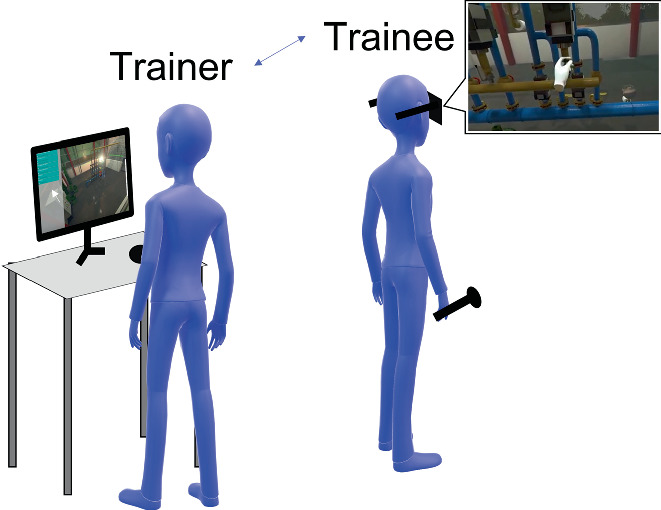
\includegraphics[width=0.7\linewidth]{figs/mr-example-collab.png}
        \caption{Collaborative setup for training in industrial scenarios using \ac{MR} \cite{Mayer2023}}
        \label{f:mr-collab-example}
    \end{figure}

    *TODO: Verify this part a bit better - clarify the distinction between the referenced collaboration scenario and the collaboration of this dissertation, can I say that the remote user sees is immersed into an VR environment that the on-site also sees? because the on-site member sees it via AR and not only VR? 
    
    Although this example highlights the collaborative potential of \ac{MR}, it slightly differs from the ideal collaboration model developed in this project. Here, the focus is on enabling an \textbf{on-site} user to interact with the real world through \ac{AR}—visualizing real-time data overlaid onto their physical environment—while the \textbf{remote} user experiences the same \ac{VR} environment. This configuration allows the remote user to be fully immersed in a virtual reconstruction of the on-site environment, with the ability to monitor and collaborate with the on-site user in real-time. The goal is not only to enhance communication but to enable mutual interaction with a shared digital-physical environment, fostering more precise decision-making, particularly in complex, dynamic tasks. This setup, more reflective of the full potential of \ac{MR}, aligns closely with Industry 5.0’s vision of combining human expertise and advanced technology for seamless collaboration between humans and machines across different realities.


    % \subsubsection{Extended Reality (\ac{XR})}
    % The term \ac{XR} serves as an umbrella concept that includes \ac{AR}, \ac{MR}, and \ac{VR} as distinct but related technologies. It encompasses technologies designed to enhance sensory experiences by blending the physical and digital worlds \cite{pesca2021augmented}. These technologies allow users to engage with virtual and augmented elements in varying degrees, depending on the specific application or device in use.


% use this? - 17 set 00h18
% Therefore, it holds great promise for enhancing collaborative efforts, particularly in remote interactions, where \ac{AR} is utilized by for 
% on-site members, overlaying digital information onto the physical environment, and \ac{VR} is employed for remote members, immersing them in 
% a simulated virtual environment. This integration of both digital realities allow participants from different locales to share a common virtual 
% space for interaction.

%%%%%%%%%%%%%%    % 16 set 18h04  a parte acima esta ok, ver so se é preciso adicionar mais alguma figura

%%%%%%%%%%%%%% é preciso entrar em mais detalhe sobre o que é MR e como se enquadra no contexto de HRC????? faz sentido? - do artigo de mixed realities
%%%%%%%%%%%%%% capitulo 8 - a conceptual framework for mixed reality . 16 set 18h04
    % \subsection*{Summary of Mixed Reality Concepts}

    % The landscape of \ac{MR} is notably fragmented, influenced by diverse expert opinions and various scholarly sources. 
    % Despite these differences, there is a consensus on the utility of a unified definition for clarity, particularly within Human-Computer Interaction 
    % research. However, the approach adopted does not seek to establish a singular definition but rather to accommodate the variety of existing perspectives.
    
    % \subsection*{Conceptual Dimensions of MR}

    % Several dimensions have been identified to classify \ac{MR} experiences more clearly:

    % \begin{itemize}
    %     \item \textbf{Number of Environments:} This dimension addresses the count of physical and virtual environments involved in \ac{MR} experiences. 
    %     For instance, a \ac{VR} experience might be considered a separate environment even when occurring in the same physical space as an \ac{AR} setup.
    %     \item \textbf{Number of Users:} Reflects the user involvement needed for different types of \ac{MR}. While the collaboration type of \ac{MR} 
    %     typically involves multiple users, other forms might not.
    %     \item \textbf{Level of Immersion:} Describes the depth of immersion, which varies independently from the level of virtuality. This is crucial 
    %     for understanding user engagement in \ac{MR} environments.
    %     \item \textbf{Level of Virtuality:} Indicates the extent of virtual content integrated into the user's perception. It parallels the 
    %     Reality-Virtuality Continuum and varies from non-existent to fully virtual.
    %     \item \textbf{Degree of Interaction:} Categorized into implicit and explicit interactions, this dimension focuses on how users interact 
    %     with the \ac{MR} system—ranging from passive engagement to active manipulation of the \ac{MR} scene.
    % \end{itemize}

    % \subsection*{Additional Dimensions}

    % \begin{itemize}
    %     \item \textbf{Input:} Encompasses non-interactive inputs like motion tracking, geolocation, and sensor data, which inform the \ac{MR} environment.
    %     \item \textbf{Output:} Involves the types of sensory feedback provided to the user, potentially including visual, auditory, haptic, and other sensory outputs.
    % \end{itemize}

    % These dimensions form a framework that allows for a structured classification and discussion of \ac{MR} experiences, accommodating the range of definitions and applications highlighted by industry and academic experts.

% \subsection{Extended Reality}  -------------- perguntar ao eurico e bernardo se é preciso falar disto ou fica apenas pela mixed reality?
% % - importante para a industria 4.0
% % mencionar áreas de aplicacao onde ja existe.
% % dar + enfase aos trabalho alinhados com HRC e HRI
% \ac{XR} is a recent comprehensive term that encapsulates all immersive technologies, including \ac{VR}, \ac{AR}, and \ac{MR}. 
% These technologies extend the spectrum of human experience by merging the digital and physical realms in various degrees and forms. 

% \ac{XR} technologies are pivotal in:
% \begin{itemize}
%     \item creating a continuum of immersive experiences, ranging from fully virtual environments to the enhancement of the physical world with 
%     digital overlays \cite{Morimoto2022}.
%     \item transforming the manufacturing industry by enhancing visualization, training, and operational efficiency.
% \end{itemize} 

% \subsection{Limitations of XR}

% While \ac{XR} holds great promise for revolutionizing remote interactions, it also has challenges, especially in distant settings.

% It begins with the limitation in perspective and environmental context. The view available to remote participants is restricted to what their on-site 
% counterparts can share, which may limit a full understanding of the environment. This constraint can lead to less effective guidance and decision-making 
% from afar. 

% Moreover, \ac{XR} technologies often emphasize sharing visual and audio data, neglecting the collection of multisensory information. 
% This lack of comprehensive data collection prevents remote participants from fully grasping the nuances of the physical location, missing out 
% on critical contextual cues necessary for a deep understanding of on-site conditions.

% Additionally, the interaction with physical objects through \ac{XR} can be superficial, lacking the depth needed for intricate explanations or 
% precise gestures, especially in complex or dynamic situations. This limitation can make it challenging to perform tasks that require detailed 
% manipulation.

% Furthermore, navigation poses another challenge for on-site users, particularly in environments that are complex or fraught with hazards. 
% The difficulty in moving safely and efficiently through such spaces can compromise the sharing of contextual information and hinder the overall 
% effectiveness and efficiency of the tasks being done.

% These limitations underscore the need for ongoing advancements in \ac{XR} technology to address these gaps and fully leverage its potential in 
% remote collaboration \cite{Lambrecht2021,Suzuki2022}.



%%%%%%%%%%%%%%%%%%%%%%%%%%% abaixo - verificar se alguma informacao daqui pode ser util para os DT - 19 set 16h11 %%%%%%%%%%%%%%%%%%%%%%%%%%% 

% 19 set 00h14 - parte dos dt parece estar ok (falta adicionar figuras e tabelas) - ordenar melhor ( ver o que o chat deu)
% - a seguir falar das solucoes industriais - ar e dt para remote collaboration
% introduzir human robot collaboration antes? 
% \section{Digital Twins}
% cite from article - "state of art survey digital twin implementations" 

% \ac{DT} are virtual replicas of physical entities, enabling the simulation, analysis, and control of systems in a digital realm. 
% Their importance in enhancing \ac{HRC} lies in their ability to provide a real-time, interactive environment that mirrors the 
% physical world, allowing for improved decision-making, efficiency, and flexibility in industrial applications.

% By transforming smart manufacturing, \ac{DT} enable comprehensive examination and prediction of physical systems' behaviors, 
% optimizing operations and minimizing downtime. In \ac{HRC}, \ac{DT} significantly boost ergonomic interactions, adapting robotic movements to meet 
% human needs and constraints, thereby ensuring a safer and more productive workplace \cite{Tao2019}.

% The integration of \ac{DT} in various fields is supported by advancements in big data and \ac{IoT}, providing the necessary infrastructure for its 
% implementation. As a cutting-edge technology, \ac{DT} leverages modern data surges to assist engineers, managers, healthcare professionals, and 
% policymakers in managing complex systems such as production lines, healthcare, and smart cities (citar 4-8 confirmar quais os casos aplicaveis aqui).
% These systems offer high fidelity monitoring, diagnostics, and prognostics tools, enhancing operational oversight and decision-making processes.

% Moreover, \ac{DT} are instrumental in the proactive management of \ac{HRC}, fostering mutual-cognitive, predictable, and self-organizing functionalities that 
% enhance the efficiency and safety of \ac{HRI} \cite{Li2023}.

% Originally conceptualized by NASA in the 1980s, the idea of \ac{DT} was intended to monitor spacecrafts from Earth. This concept has evolved significantly 
% with the advancements in computational and \ac{IoT} technologies. Modern \ac{DT} systems utilize real-time data from sensors to accurately reflect the 
% state of the physical twin, enhancing the fidelity and applicability of simulations (cite 10).

% Nowadays, a notable implementation of \ac{DT} technology is observed in Singapore's Smart Nation Initiative, where the Land Transport Authority is developing a 
% \ac{DT} of the country to inform policy decisions by testing potential policies virtually before they are enacted. This application not only demonstrates
% the immense potential of \ac{DT} for contemporary and future technologies but also underscores the ongoing commitment to advancing this concept (cite 6).

% However, the concept of \ac{DT} lacks a standardized definition, leading to a variability in the scope and execution of \ac{DT} implementations. 
% The dual nature of cyber and physical components in \ac{DT} makes \ac{AR} a suitable companion for visualizing and interacting with these complex 
% systems (cite the article itself).

% As \ac{DT} technology continues to attract interest, the necessity for intuitive data visualization methods becomes apparent. Non-expert users must 
% be able to understand and interact with the complex data provided by \ac{DT} systems effectively. \ac{AR} offers a promising solution by overlaying 
% virtual data directly onto physical objects, providing a more natural and intuitive user interface for interacting with digital 
% information cite(12).
% \ac{AR} expands the traditional interaction from 2D screens to 3D real-world applications, making it an ideal tool for enhancing user interaction 
% with digital twins. By enabling users to view and interact with maintenance instructions projected directly onto equipment, \ac{AR} facilitates more 
% efficient and effective operation and maintenance processes (cite 13).



% \subsection*{Digital Twins in Academia and Industry}
% The term \ac{DT} is widely recognized in both academic and industrial circles as a \ac{CPS} that typically consists of three main components: 
% \begin{itemize}
%     \item A physical system.
%     \item A virtual model.
%     \item The connections between them (cite 1,2,3 from the dt article).
% \end{itemize}

% Research applications of \ac{DT} span across 
% various fields, offering solutions for lifecycle management, \ac{PHM}, and urban planning, to name a few (cite 4-8).

% Critically, the industry's adoption of \ac{DT}, led by companies like Siemens, often focuses on creating digital shadows rather than true \ac{DT}, 
% characterized by a lack of bidirectional communication. True \ac{DT} systems are distinguished by their ability to not only update the virtual model 
% based on changes in the physical system but also to allow alterations in the virtual model to affect the physical entity (cite 9- add table 5).

%%%%%%%%%%%%%%%%%%%%%%%%%%% acima - verificar se alguma informacao daqui pode ser util para os DT - 19 set 16h11 %%%%%%%%%%%%%%%%%%%%%%%%%%% 

%%%%%%%%%%%%%%%%%%%%%%%%%%% abaixo - parte a usar para DT - 19 set 16h11 %%%%%%%%%%%%%%%%%%%%%%%%%%%%%%%%%%%%%%%%%%%%%%%%%%%%%%  

\section{Digital Twins}
\label{sec:dt}
Another relevant concept are \ac{DTs}, which consist on sophisticated digital replicas of physical entities, allowing for the simulation, analysis, and control of systems within a digital framework. These digital counterparts have emerged as pivotal technologies in a variety of domains, particularly in enhancing \ac{HRC}, as they offer real-time, interactive environments that mirror physical systems. The ability to replicate physical entities with high fidelity enables improved decision-making, operational efficiency, and flexibility across a wide range of industrial applications.
*TODO: add a reference above

This \ac{DT} concept was first introduced by NASA in the 1980s as part of its spacecraft monitoring systems, where virtual models were employed to replicate the conditions and behavior of spacecraft during missions. Over the past decades, advances in \ac{IoT}, sensor technology, and computational power have significantly improved the capabilities of \ac{DTs}, moving beyond their original use case. Modern systems leverage real-time sensor data and advanced simulation techniques to enhance the accuracy and reliability of digital models, enabling more sophisticated predictions, real-time analytics, and simulations of complex systems \cite{liu2022digitaltwin}.

In current manufacturing and industry scenarios, \ac{DTs} play a transformative role, particularly in smart manufacturing systems, where they enable detailed examination and prediction of the behavior of physical systems. This capability allows companies to optimize operations, reduce downtime, and improve overall system efficiency. Furthermore, in \ac{HRC}, \ac{DTs} facilitate safer and more productive work environments by dynamically adjusting robotic movements and operations to better align with human needs, thereby enhancing ergonomic interactions and mitigating safety risks \cite{8477101}.

A prominent real-world implementation of this technology is seen in Singapore's Smart Nation Initiative, where the Land Transport Authority employs a \ac{DT} to simulate and evaluate potential policy decisions before their implementation. This application exemplifies the wide-ranging potential of \ac{DTs} to support decision-making processes in urban planning, infrastructure management, and beyond \cite{isprs-archives-XLII-4-W7-37-2017}. As these technologies evolve, their applications in both academic research and industrial practice are rapidly expanding.

The academic landscape surrounding \ac{DTs} has seen extensive research exploring their versatility and potential, having been applied to a broad spectrum of areas, illustrating the profound impact of DTs on enhancing system efficiency, predictive maintenance, and overall operational performance \cite{8361285, TAO2018169, isprs-archives-XLII-4-W7-37-2017, 10.1007/978-3-030-23162-0_19, 6296978}.
*TODO: usar uma destas referencias para pôr no paragrafo introdutorio sobre os DTs.

Despite the growing prominence of \ac{DTs}, there is still no universally accepted formal definition of the concept. However, most scholars and industry experts concur that a \ac{DT} is a type of \ac{CPS} consisting of three fundamental components: a physical system, a virtual model, and bidirectional communication between these two models \cite{TaoFei, 8477101, ROSEN2015567}.
This interaction is fundamental to the operation of true \ac{DTs}, allowing for a continuous feedback loop where changes in the physical world can inform the virtual model, and, in turn, decisions or optimizations made in the digital realm can directly influence the physical system.

In contrast to true \ac{DTs}, some critics argue that many commercially available implementations, such as those provided by companies like Siemens, represent "digital shadows" rather than full \ac{DTs}. The distinction lies in the capability for bidirectional communication. In many digital shadow systems, changes in the physical system are reflected in the virtual model, but there is no capacity for the virtual model to directly control or alter the physical system. This one-way communication limits the interactive and predictive capabilities that define a true DT \cite{CIMINO2019103130}.

To illustrate the distinction, Figure \ref{f:dt-structure} presents a reference model of a \ac{DT}, showcasing the bidirectional flow of information between physical and digital entities. This structure is essential for enabling real-time interaction and feedback, core characteristics that  differentiate \ac{DTs} from digital shadows. True \ac{DTs} must facilitate a continuous, reciprocal exchange of data between physical and virtual domains, allowing the virtual model to reflect and affect the physical system \cite{dt_model}.

\begin{figure}[!htpb]
    \centering
    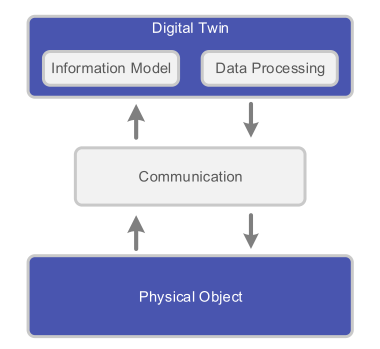
\includegraphics[width=0.4\linewidth]{figs/dt_reference_model.png}
    \caption{A Digital Twin reference model, emphasizing the importance of bidirectional communication between the physical object and its digital counterpart~\cite{dt_model}}
    \label{f:dt-structure}
\end{figure}

Bidirectional communication's importance in \ac{DTs} is further emphasized by Liu et al.~\cite{liu2022state}, who argue that “a true DT must include bidirectional communication instead of having a virtual model that only updates according to a physical system.” This distinction between the types of communication and interaction is critical, as it defines the extent to which a \ac{DT} can be leveraged for control, simulation, and predictive purposes.

Table \ref{tab:levels_of_control} outlines different interaction levels within \ac{DT} systems, ranging from no interaction, where the physical and virtual systems are disconnected, to unidirectional data flow, where data is transferred from the physical to the virtual model, and culminating in bidirectional communication. The latter represents a fully functional \ac{DT}, where continuous exchange of data allows the virtual model to influence and control the physical system, achieving real-time synchronization and interaction.

% Table \ref{tab:levels_of_control} illustrates interaction levels present in \ac{DT} systems, from no interaction, to unidirectional data flow, and ultimately to bidirectional communication, the latest defining a fully functional \ac{DT}.

\begin{table}[!htpb]
    \centering
    \caption{Levels of Interaction in a Digital Twin system between the physical model and its digital counterpart, adapted from \cite{liu2022state}}
    \label{tab:levels_of_control}
    \begin{tabular}{@{}l>{\raggedright\arraybackslash}p{10cm}@{}}
    \toprule
    Level of Interaction & Description \\ 
    \midrule
    No interaction & Virtual model and physical system are not connected through a network. The virtual model only simulates and models a physical 
    system without any real-time updates. \\ \hline
    Unidirectional & The physical system feeds sensor data to the virtual model through a network. The virtual model utilizes data to update the 
    current state and predict future states. \\ \hline
    Bidirectional & Both the physical system and the virtual model can send data to each other. The virtual model updates using physical data while 
    the physical system can be controlled through data sent by the virtual model. \\ 
    \bottomrule
    \end{tabular}
\end{table}


\section{Human-Robot Collaboration in Industrial Applications}
\label{sec:hrc-in-industry}
Following the detailed exploration of \ac{DT} and \ac{MR}, this section discusses how these technologies integrate into \ac{HRC}, demonstrating significant improvements in interaction, safety and efficacy in practical examples from industry solutions with specific emphasis on remote collaboration.

The articles cited below often reference \ac{AR}, however, it is important to note that in many cases, the features described under \ac{AR} align more closely with the concept of \ac{MR} as a medium for collaboration, as explained in \ref{subsection:digital-realities}. This distinction is crucial, as the developed system is more aligned with \ac{MR}’s capability to further facilitate shared virtual and physical environments, enhancing interaction and collaborative processes across industrial applications.

\subsection{Enhancing Human-Robot Collaboration through Augmented Reality and Digital Twin Implementation}
 
Chu et al.~\cite{CHU2023313} reviewed various studies on integrating \ac{AR} with \ac{DT} to improve \ac{HRC} using visual and haptic feedback interfaces. Their work emphasizes the value of \ac{AR} in enhancing human-robot communication by providing both egocentric (shared remote views) and exocentric (spatial visualization of the robot relative to the workspace) perspectives, thereby improving spatial awareness and interaction quality. 

Green et al.~\cite{doi:10.5772/5664} further highlight that multimodal \ac{AR} interfaces—incorporating visual, haptic, and acoustic cues—can significantly enhance \ac{HRC}. Multimodal approaches help overcome challenges like limited \ac{FOV} in \ac{HMDs}, making the interaction more intuitive. For instance, audio-tactile feedback is particularly beneficial for individuals with visual impairments, providing alternative sensory channels without compromising performance. Visual \ac{AR} cues, implemented through \ac{HMDs}, help users navigate complex environments by overlaying relevant information, thus enhancing navigation without impeding robotic movement.

Lasota et al.~\cite{doi:10.1177/0018720814565188} conducted experiments to evaluate the impact of human-aware motion planning on \ac{HRC}, demonstrating substantial improvements in task performance and team fluency. Compared to standard robotic systems, participants working with human-aware robots completed tasks more efficiently, exhibited greater concurrent motion, and experienced less idle time for both human and robot. Moreover, they maintained greater separation distances, which reduced collision risks and increased perceived safety. These results illustrate the dual advantage of human-aware planning: it not only enhances task efficiency but also elevates worker comfort and safety, which are critical for minimizing stress-related risks in industrial environments.

The study utilized the \ac{ROS} to control a WidowX 250 Robot Arm, using the MoveIt framework for motion planning. This approach ensures modularity, adaptability, and ease of management in shared \ac{HRC} environments. Both \ac{AR} and \ac{DT} models were developed using the Microsoft HoloLens 2 for visual feedback and the SenseGlove Nova™ for haptic feedback, offering a comprehensive multimodal experience.

Through the HoloLens, users could visualize the robot's planned trajectory and swept volume, thus anticipating its actions. Concurrently, the haptic interface provided vibration feedback to signal the robot's proximity and target destinations, as illustrated in Figure~\ref{fig:haptic-visual-cues}. These multimodal cues offered varying levels of detail, aiding coordination in tasks that required awareness of robot movements.

\begin{figure}[htp]
    \centering
    \begin{subfigure}{\textwidth}
        \centering
        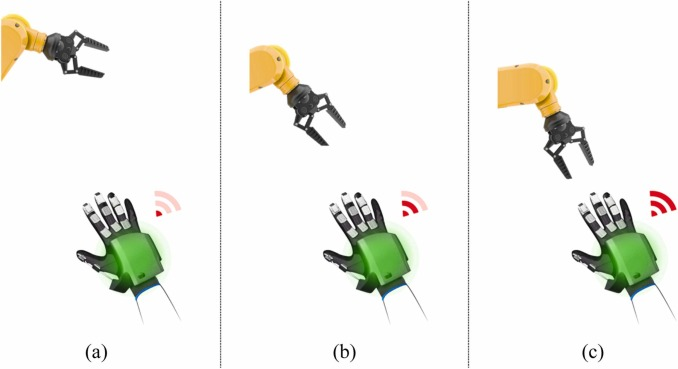
\includegraphics[width=0.6\linewidth]{figs/haptic-cues.jpg}
        \caption{Cues indicating the gripper’s destination using vibration on different human fingers.}
        \label{fig:sfig1}
    \end{subfigure}

    \vspace{0.5cm} % Adds space between the figures
    
    \begin{subfigure}{\textwidth}
        \centering
        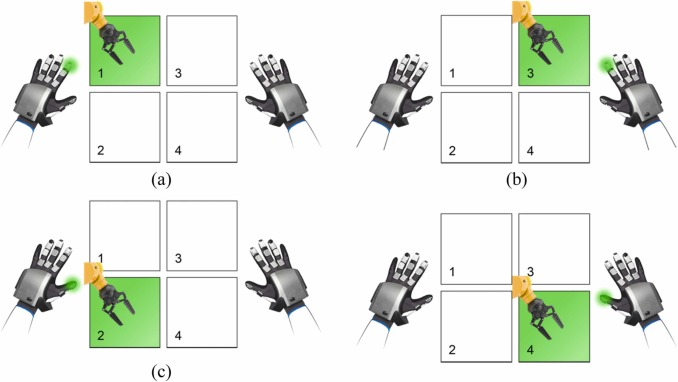
\includegraphics[width=0.6\linewidth]{figs/visual-cues.jpg}
        \caption{Cues indicating the proximity of the gripper via vibration frequency changes.}
        \label{fig:sfig2}
    \end{subfigure}
    
    \caption{Visual and haptic interfaces used in the experiment~\cite{CHU2023313}.}
    \label{fig:haptic-visual-cues}
\end{figure}

% \subsubsection{Benefits of Multimodal Feedback}

Findings show that combining visual, haptic, and acoustic cues significantly improve task performance. Visual interfaces, especially those indicating proximity, excelled in usability, while haptic feedback proved invaluable in scenarios where visual input was insufficient or overloaded. Acoustic signals also served as alerts for sudden changes in the robot's motion, helping reduce operator anxiety in unpredictable environments.

In a task where the operator and robot worked independently but in close proximity, the system enabled efficient coordination. The robot delivered materials while the operator performed assembly tasks, highlighting the potential for \ac{AR}-based interfaces to optimize \ac{HRC} in industrial settings.


% %%%%%%%%%%%%%%%%%%%%% previous version %%%%%%%%%%%%%%%%%%%%%
% \subsection{Augmented Reality-Assisted Multi-Robot Systems for Enhanced Control and Coordination}
% % below, update the correct references
% Integrating \ac{AR} into multi-robot manufacturing systems offers significant improvements in interaction, operational safety, and efficiency, especially when applied to real-time and planned control modes.

% Ong et al.~\cite{ong2020} further explored \ac{AR}-assisted robot programming for welding applications, demonstrating that user-friendly interfaces can significantly reduce the complexity and duration of the programming process. These interfaces enable operators to define welding points and orientations using handheld pointers, thus enhancing task accuracy and efficiency by allowing validation within the actual robot workspace.

% Malí et al.~\cite{7819154} developed an \ac{AR} application that permits users to adjust robot axis values, visualize specific robot points through 3D arrows, and navigate hidden points using leading lines. Evaluated in an industrial setting, this application showed improvements in usability and interaction capabilities.

% Puljiz et al.~\cite{puljiz2019conceptsendtoendaugmentedreality,puljiz2} explored various \ac{AR}-based methods for robotic arm programming using devices like the Microsoft HoloLens, implementing techniques such as hand-guided task programming, augmented trajectory visualization, and the creation of spatial maps for virtual waypoint placement. These methods facilitate intuitive and accurate robotic arm programming, enabling seamless integration between virtual commands and real-world operations.

% Modern manufacturing trends are characterized by a shift toward mass customization and increased flexibility, driven by the demand for individualized products. This necessitates more adaptable manufacturing systems where human operators collaborate with industrial robots to handle complex tasks~\cite{1-ar-dt,2-ar-dt,3-ar-dt}. However, existing robotic systems primarily execute pre-programmed tasks with limited intelligence.

% To address this, two promising approaches have emerged: leveraging advanced \ac{AI} techniques for robot learning~\cite{6-ar-dt} and integrating a human-in-the-loop strategy for robot teleoperation. The latter, more aligned with Industry 5.0 principles, extends the capabilities of both humans and robots by incorporating human expertise into collaborative multi-robot processes~\cite{7-ar-dt}.

% Unlike traditional \ac{HRC}, multi-robot manufacturing with a human in the loop allows operators to interact with robots from remote locations, not limited to physical workspaces. This paradigm facilitates safer and more flexible manufacturing, by bridging the gap between fully automated and manual operations~\cite{7-ar-dt}. However, significant challenges remain, including the need for more user-friendly teleoperation interfaces and systems that can be easily utilized by manufacturing operators without extensive robotics training~\cite{9-ar-dt}.

% Research in multi-agent collaborative manufacturing has focused on enhancing safety, productivity, and cost reduction. Wearable \ac{AR}-assisted systems and \ac{DT} technologies enable accurate and intuitive robot teleoperation. By combining \ac{AR} with robot teleoperation, workers can access physical and virtual information simultaneously in a hybrid environment, interacting with virtual objects~\cite{26-ar-dt,27-ar-dt}. An example is an \ac{AR}-based teleoperation system utilizing RGB-D imaging, allowing operators to perceive the remote robot's environment and perform teleoperation~\cite{10-ar-dt}. Another system transforms robot workspaces into \ac{AR} environments for rapid and intuitive path planning and task programming~\cite{30-ar-dt}. These systems improve task performance by providing additional visual cues to enhance the operator's situational awareness.

% Recent advancements in smart manufacturing have led to the development of \ac{DT} models for robot control. For example, \cite{37-ar-dt} used the Unity engine to create a \ac{DT} of a robot arm that could learn manufacturing tasks virtually and replicate them in the physical world. The integration of \ac{DT} and \ac{VR} interfaces has also been proposed to design immersive human-in-the-loop robotic systems, where the \ac{DT} acts as an intermediary layer for task execution and quality monitoring~\cite{41-ar-dt,42-ar-dt}.

% Li et al.~\cite{LI2022102321} demonstrated how \ac{AR}-assisted \ac{DTs} enable operators to manage and coordinate multiple robots more effectively.
% Figure~\ref{fig:physical-digital} depicts an immersive dual view where users can interact with the physical setup of two collaborating robots while simultaneously observing their virtual counterparts through Microsoft HoloLens \ac{AR} glasses. This setup allows for real-time monitoring and simulation of manufacturing processes, improving robot operation control.

% \begin{figure}[!htpb]
%     \centering
%     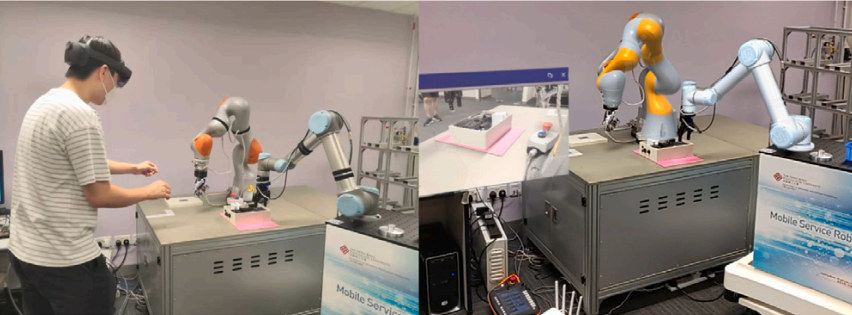
\includegraphics[width=0.85\linewidth]{figs/physical-digital.png}
%     \caption{\ac{AR}-assisted \ac{DT}-enabled multi-robot collaborative manufacturing system \cite{LI2022102321}.}
%     \label{fig:physical-digital}
% \end{figure}

% Their proposed comprehensive framework for an \ac{AR}-assisted, \ac{DT}-enabled robot collaborative manufacturing system features human-in-the-loop control. The system architecture, shown in Figure~\ref{f:system-framework}, introduces a multi-node communication mechanism to facilitate interactions among multiple robots and clients. It includes the design of an \ac{AR}-based teleoperation system for pose registration and motion planning, coupled with three \ac{DT}-enabled interaction approaches to achieve closed-loop interaction between virtual and physical robots.

% \begin{figure}[!htpb]
%     \centering
%     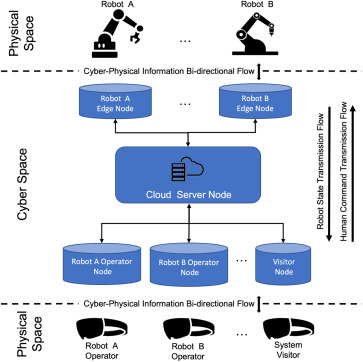
\includegraphics[width=0.5\linewidth]{figs/framework.jpg}
%     \caption{The architecture of a multi-robot, multi-client communication mechanism \cite{LI2022102321}.}
%     \label{f:system-framework}
% \end{figure}

% The \ac{DT} of the physical robot, modeled using the Unity engine, is displayed as a hologram in the remote workspace via \ac{AR} glasses, enabling teleoperation and remote monitoring. Pose registration involves aligning the virtual and physical robot models using the Vuforia Engine, while joint alignment translates \ac{DT} joint values into real-world coordinates.

% Therefore, a robot control approach aided by \ac{AR} technology offers several benefits:
% \begin{itemize}
%     \item Enhanced predictability of robot posture and motion trajectories.
%     \item Trajectory visualization to prevent safety issues.
%     \item An intuitive interface that overcomes spatial and physical limitations.
% \end{itemize}

% However, observing workspace and robot state information during task execution presents challenges, such as networking latency and positioning accuracy. Proposed solutions include time-sensitive networks and advanced communication technologies such as 5G~\cite{LI2022102321}.

% The proposed system utilizes IP cameras for workspace monitoring, projecting video feeds onto \ac{AR} glasses for enhanced remote monitoring, as shown in Figure~\ref{f:workspace-visualization}.

% \begin{figure}[!htpb]
%     \centering
%     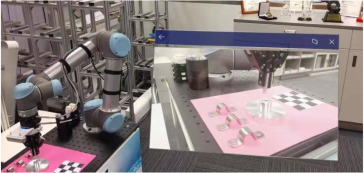
\includegraphics[width=0.7\linewidth]{figs/workspace-visualization.jpg}
%     \caption{Demonstration of the workspace observation approach \cite{LI2022102321}.}
%     \label{f:workspace-visualization}
% \end{figure}
% \FloatBarrier


% Despite these advancements, challenges such as \ac{DT} model accuracy and network latency still affect the overall system performance. Addressing these limitations is essential for realizing the full potential of \ac{AR}-assisted \ac{DT} systems in industrial applications~\cite{LI2022102321}.

% do a conclusion of the state of art. i will transition into the methodology of proposing the system - taking into consideration several aspects of the state of art such as: using Unity 3D for robot model development, trying to implement the billateral communication of digital twins by utilizing a robot that already has \ac{ROS} working on it as well as the packages that allow it to move. besides that, the use of vuforia to do the pose registration of the robot. The suggestions of the visual and audio cues that can be implemented in AR.  the safety-zone interactions allow the user to be aware of the robot's movements and prevent accidents, as well as the audio implemented - these are great ideas.
% the robot manipulation was implemented in an easy to understand by non-experient people, were implemented from the remote site - unity - by utilizing the Interface of an HHD device to manipulate each joint separately -  by pressing a publish button that will send the robot to the desired real location.
%  from the \ac{ROS} side, by manipulating the robot through its console, unity digital twin will be updated in real time, and the robot position will be visible for the remote user by visualizing the robot's position in the HHD device.
% the camera feed transmition is also good to mention because it allows the remote user to visualzie the workspace that is being worked on.

% do a conclusion of the state of art.

% \end{enumerate}

% either this one or the below one

\subsection{Augmented Reality-Assisted Multi-Robot Systems for Enhanced Control and Coordination}

Integrating \ac{AR} into multi-robot manufacturing systems offers significant improvements in interaction, operational safety, and efficiency, especially when applied to real-time and planned control modes. Ong et al.~\cite{ong2020} further explored \ac{AR}-assisted robot programming for welding applications, demonstrating that user-friendly interfaces can significantly reduce the complexity and duration of the programming process. These interfaces enable operators to define welding points and orientations using handheld pointers, thus enhancing task accuracy and efficiency by allowing validation within the actual robot workspace.

Malí et al.~\cite{7819154} developed an \ac{AR} application that permits users to adjust robot axis values, visualize specific robot points through 3D arrows, and navigate hidden points using leading lines. Evaluated in an industrial setting, this application showed improvements in usability and interaction capabilities.

Puljiz et al.~\cite{puljiz2019conceptsendtoendaugmentedreality,puljiz2} explored various \ac{AR}-based methods for robotic arm programming using devices like the Microsoft HoloLens, implementing techniques such as hand-guided task programming, augmented trajectory visualization, and the creation of spatial maps for virtual waypoint placement. These methods facilitate intuitive and accurate robotic arm programming, enabling seamless integration between virtual commands and real-world operations.

Modern manufacturing trends are characterized by a shift toward mass customization and increased flexibility, driven by the demand for individualized products. This necessitates more adaptable manufacturing systems where human operators collaborate with industrial robots to handle complex tasks~\cite{1-ar-dt,2-ar-dt,3-ar-dt}. However, existing robotic systems primarily execute pre-programmed tasks with limited intelligence.

To address this, two promising approaches have emerged: leveraging advanced \ac{AI} techniques for robot learning~\cite{6-ar-dt} and integrating a human-in-the-loop strategy for robot teleoperation. The latter, more aligned with Industry 5.0 principles, extends the capabilities of both humans and robots by incorporating human expertise into collaborative multi-robot processes~\cite{7-ar-dt}.

Unlike traditional \ac{HRC}, multi-robot manufacturing with a human in the loop allows operators to interact with robots from remote locations, not limited to physical workspaces. This paradigm facilitates safer and more flexible manufacturing, by bridging the gap between fully automated and manual operations~\cite{7-ar-dt}. However, significant challenges remain, including the need for more user-friendly teleoperation interfaces and systems that can be easily utilized by manufacturing operators without extensive robotics training~\cite{9-ar-dt}.

Research in multi-agent collaborative manufacturing has focused on enhancing safety, productivity, and cost reduction. Wearable \ac{AR}-assisted systems and \ac{DT} technologies enable accurate and intuitive robot teleoperation. By combining \ac{AR} with robot teleoperation, workers can access physical and virtual information simultaneously in a hybrid environment, interacting with virtual objects~\cite{26-ar-dt,27-ar-dt}. An example is an \ac{AR}-based teleoperation system utilizing RGB-D imaging, allowing operators to perceive the remote robot's environment and perform teleoperation~\cite{10-ar-dt}. Another system transforms robot workspaces into \ac{AR} environments for rapid and intuitive path planning and task programming~\cite{30-ar-dt}. These systems improve task performance by providing additional visual cues to enhance the operator's situational awareness.

Recent advancements in smart manufacturing have led to the development of \ac{DT} models for robot control. For example, \cite{37-ar-dt} used the Unity engine to create a \ac{DT} of a robot arm that could learn manufacturing tasks virtually and replicate them in the physical world. The integration of \ac{DT} and \ac{VR} interfaces has also been proposed to design immersive human-in-the-loop robotic systems, where the \ac{DT} acts as an intermediary layer for task execution and quality monitoring~\cite{41-ar-dt,42-ar-dt}.

Li et al.~\cite{LI2022102321} demonstrated how \ac{AR}-assisted \ac{DTs} enable operators to manage and coordinate multiple robots more effectively.
Figure~\ref{fig:physical-digital} depicts an immersive dual view where users can interact with the physical setup of two collaborating robots while simultaneously observing their virtual counterparts through Microsoft HoloLens \ac{AR} glasses. This setup allows for real-time monitoring and simulation of manufacturing processes, improving robot operation control.

\begin{figure}[!htpb]
    \centering
    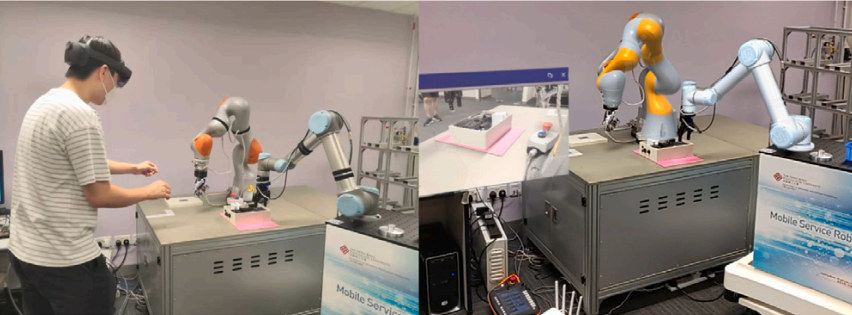
\includegraphics[width=0.85\linewidth]{figs/physical-digital.png}
    \caption{\ac{AR}-assisted \ac{DT}-enabled multi-robot collaborative manufacturing system~\cite{LI2022102321}.}
    \label{fig:physical-digital}
\end{figure}

Their proposed comprehensive framework for an \ac{AR}-assisted, \ac{DT}-enabled robot collaborative manufacturing system features human-in-the-loop control. The system architecture, shown in Figure~\ref{f:system-framework}, introduces a multi-node communication mechanism to facilitate interactions among multiple robots and clients. It includes the design of an \ac{AR}-based teleoperation system for pose registration and motion planning, coupled with three \ac{DT}-enabled interaction approaches to achieve closed-loop interaction between virtual and physical robots.

\begin{figure}[!htpb]
    \centering
    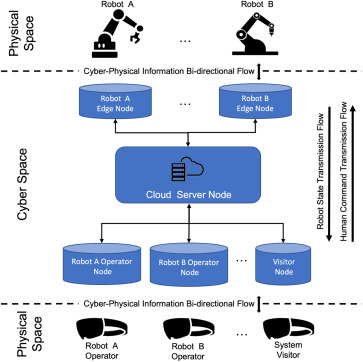
\includegraphics[width=0.5\linewidth]{figs/framework.jpg}
    \caption{The architecture of a multi-robot, multi-client communication mechanism~\cite{LI2022102321}.}
    \label{f:system-framework}
\end{figure}

The \ac{DT} of the physical robot, modeled using the Unity engine, is displayed as a hologram in the remote workspace via \ac{AR} glasses, enabling teleoperation and remote monitoring. Pose registration involves aligning the virtual and physical robot models using the Vuforia Engine, while joint alignment translates \ac{DT} joint values into real-world coordinates.

Therefore, a robot control approach aided by \ac{AR} technology offers several benefits:
\begin{itemize}
    \item Enhanced predictability of robot posture and motion trajectories.
    \item Trajectory visualization to prevent safety issues.
    \item An intuitive interface that overcomes spatial and physical limitations.
\end{itemize}

However, observing workspace and robot state information during task execution presents challenges, such as networking latency and positioning accuracy. Proposed solutions include time-sensitive networks and advanced communication technologies such as 5G~\cite{LI2022102321}.

The proposed system also utilizes IP cameras for workspace monitoring, projecting video feeds onto \ac{AR} glasses for enhanced remote monitoring, as shown in Figure~\ref{f:workspace-visualization}.

\begin{figure}[!htpb]
    \centering
    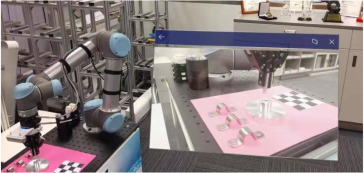
\includegraphics[width=0.7\linewidth]{figs/workspace-visualization.jpg}
    \caption{Demonstration of the workspace observation approach~\cite{LI2022102321}.}
    \label{f:workspace-visualization}
\end{figure}
\FloatBarrier


% Despite these advancements, challenges such as \ac{DT} model accuracy and network latency still affect the overall system performance. Addressing these limitations is essential for realizing the full potential of \ac{AR}-assisted \ac{DT} systems in industrial applications~\cite{LI2022102321}.


\section{Future Trends in Human-Robot Collaboration}

All in all, future directions in \ac{HRC} are evolving due to advancements in cobot technologies, sensing methodologies, and algorithmic developments \cite{robotics8040100}. The key trends identified include:

\begin{itemize}
    \item \textbf{Enhanced Scene Understanding:} Next-generation \ac{HRC} systems will prioritize deeper contextual awareness of the workspace and tasks at hand. This involves not only detecting the physical environment but also interpreting operator intentions, recognizing task progression, and continuously monitoring environmental dynamics. Such enhanced scene understanding will enable robots to anticipate human actions, predict potential safety risks, and adjust their behavior accordingly, thus fostering a higher level of operational safety and efficiency.

    \item \textbf{Advanced Sensing and Data Fusion:} To facilitate this enhanced scene understanding, advanced sensing methodologies and sophisticated data fusion techniques will be critical. By integrating multi-modal sensor data—such as visual, tactile, and auditory inputs—robots will be able to construct more comprehensive models of their surroundings and human collaborators. Real-time fusion of such data will allow systems to process information more effectively, ensuring safer interactions by predicting hazardous movements and improving overall system transparency. This, in turn, will enhance user trust and accelerate the adoption of \ac{HRC} solutions across industries.

    \item \textbf{Improved Task Planning and Adaptive Learning:} Future \ac{HRC} systems will be distinguished by advanced task planning capabilities, driven by more sophisticated task modeling and real-time adaptation mechanisms. As robots become more capable of autonomously learning from both structured and unstructured environments, their ability to handle a wider array of tasks will expand, reducing human involvement in routine planning stages. The deployment of these capabilities in manufacturing and service sectors will enable robots to shift between tasks seamlessly, dynamically adjusting their behavior to respond to real-time changes in production or workflow.

    \item \textbf{User-Friendly Interfaces and Interaction Methods:} As the complexity of \ac{HRC} systems increases, the need for intuitive and accessible human-robot interfaces will become paramount. Developing user interfaces that enable seamless human control without requiring advanced technical expertise is a key area of research. Implementing \ac{AR} and \ac{VR} technologies is expected to play a pivotal role in this domain, offering operators immersive and intuitive control mechanisms. These interfaces will reduce cognitive load and enable operators to interact with robots more effectively, thus improving operational efficiency and overall system usability.

    \item Among other relevant topics, which will not be further described due to not being the focus of this dissertation, incorporating \ac{ML} and adaptive learning algorithms into \ac{HRC} systems also represent a transformative leap forward.
    %  Techniques such as learning-by-demonstration, and \ac{RL} will enable robots to more accurately mimic human dexterity and decision-making processes, allowing them to learn from human input and adapt to non-repetitive, complex tasks. These adaptive systems will continuously improve based on interaction data, leading to more intuitive and efficient \ac{HRC} in dynamic industrial environments.
\end{itemize}


Historically, the focus has been on increasing the relevance of \ac{HRI} by addressing higher safety requirements and enabling 
robots to perform more complex tasks. Recently, the scope has expanded to include more sophisticated methods aimed at enhancing system performance, 
applying these methods across different application fields and tackling more intricate tasks. This expansion is driven by the emergence of new 
cobots, advancements in sensing technologies, matured algorithms, and accumulated experience in designing collaborative workcells \cite{robotics8040100}.

\section{Summary}

Even though significant advancements in \ac{AR}-\ac{DT} implementations over the past decade, the state-of-the-art literature predominantly focuses on developing applications for on-site personnel. Remote collaboration, particularly in \ac{HRC} scenarios, has received comparatively less attention, highlighting the need for systems that effectively facilitate both on-site and remote collaboration. Therefore, the proposed project aims to facilitate and integrate better remote collaboration by proposing a generalized conceptual system applicable across various application scenarios.

Despite having developed on-site features, such as \ac{DT} pose registration alongside audio and visual cues, focus will be mainly on the remote collaboration part implementation and the billateral communication between users. Unity 3D engine will be further explored for robot model development, \ac{ROS} will be used for robot control, and Vuforia for pose registration. It will also incorporate visual and audio cues to enhance user safety and awareness, as well as \ac{MR} elements implemented with Unity 3D. A camera will enable workspace monitoring. 

In conclusion, the proposed system will enable remote users to manipulate the robot using \ac{HHD}, with the robot's real-time position displayed in the Unity \ac{DT}. By addressing these challenges, the project aims to enhance remote collaboration in \ac{HRC} scenarios, contributing to the broader field of \ac{MR}-\ac{DT} applications.


% %add this part somewhere
% from article: 9911168
% "AI, AR, DT and HRC approaches are employed in smart manufacturing to transform data processing into digital processing and controlling. 
% Therefore, designing smart systems will lead to high-quality real-time data exchange, zero wasted efforts and better data management [43]. 
% Focusing on HRC applications, HRC is the future alternative to conventional robotic and automation systems."

% %also add this part somewhere:
% from article: chang-ar-hrc
% " Augmented reality will only continue to mature into
% a more accessible technology, and its role in human–robot collaboration can become much
% more impactful and relevant to many different domains"


% from chat - use this and remove the below future work and summary? - check this
% \section{Future Trends in Human-Robot Collaboration}

% As detailed in the 2019 article \textit{Human–Robot Collaboration in Manufacturing Applications: A Review}~\cite{robotics8040100}, the future of \ac{HRC} is shaped by ongoing advancements in collaborative robot technologies, sensing techniques, and algorithmic developments. These trends are instrumental in refining how robots and humans interact and collaborate. Key areas of development include:

% \begin{itemize}
%     \item \textbf{Enhanced Scene Understanding}: Future \ac{HRC} systems will prioritize comprehensive contextual awareness, encompassing not only environmental sensing but also interpreting human intentions, task progression, and monitoring dynamic changes. This will enable robots to predict human actions, detect potential risks, and adjust behaviors in real time, significantly improving operational safety and efficiency.

%     \item \textbf{Advanced Sensing and Data Fusion}: Achieving enhanced scene understanding necessitates sophisticated sensing methodologies and multi-modal data fusion. By integrating data from visual, tactile, and auditory sensors, robots can construct more nuanced models of their surroundings and human collaborators. Real-time data fusion will enable preemptive responses to hazards, enhancing safety and transparency, which are critical for increasing user trust in \ac{HRC} systems.

%     \item \textbf{Integration of Learning Techniques}: Incorporating \ac{ML} and adaptive learning algorithms is pivotal for advancing \ac{HRC}. Techniques such as reinforcement learning and learning-by-demonstration will empower robots to mimic human dexterity, adapt to non-repetitive tasks, and continuously improve from interaction data, leading to more intuitive and efficient collaboration.

%     \item \textbf{Improved Task Planning and Adaptive Learning}: The future of \ac{HRC} will be characterized by sophisticated task planning, supported by real-time adaptation mechanisms and complex task modeling. As robots become more adept at learning from structured and unstructured environments, their ability to seamlessly transition between tasks will reduce the need for human intervention in routine planning.

%     \item \textbf{User-Friendly Interfaces and Interaction Methods}: Given the rising complexity of \ac{HRC}, developing intuitive interfaces for non-expert users is essential. The implementation of \ac{AR} and \ac{VR} technologies will facilitate immersive, intuitive interactions, reducing cognitive load and improving system usability.
% \end{itemize}

% Overall, these emerging trends indicate a shift towards more intelligent, context-aware, and adaptive \ac{HRC} systems that prioritize both operational efficiency and user experience. Historically, the focus has been on enhancing safety standards and enabling robots to perform more complex tasks. This trajectory is now expanding, driven by advancements in cobots, sensing technologies, and algorithmic improvements, alongside accumulated experience in collaborative workcell design~\cite{robotics8040100}.

% \section{Summary}

% Despite the significant progress in \ac{MR}-\ac{DT} technologies, the state-of-the-art literature largely centers on on-site applications. The potential for enhancing remote collaboration, particularly within \ac{HRC}, remains underexplored. This gap highlights the need for systems that effectively integrate on-site and remote collaboration capabilities.

% The proposed project aims to address this gap by developing a generalized conceptual framework for remote collaboration in various scenarios. While on-site features such as digital twin pose registration and multimodal cues have been implemented, the primary focus will be on advancing remote collaboration and bidirectional communication between users.

% The project will leverage the Unity 3D engine for robot model development, \ac{ROS} for robot control, and Vuforia for pose registration. Visual and audio cues will be incorporated to enhance safety and situational awareness, with \ac{MR} elements integrated using Unity 3D. Additionally, a camera will provide workspace monitoring.

% Ultimately, the proposed system will empower remote users to manipulate the robot through \ac{HHD}, with real-time feedback displayed on the digital twin in Unity. By addressing these challenges, the project aims to advance remote collaboration in \ac{HRC}, contributing to the broader field of \ac{MR}-\ac{DT} applications.




